%--------------------------------------------------------------------------%
%                                                                          %
%               PREAMBLE                                                   %
%                                                                          %
%--------------------------------------------------------------------------%
\documentclass[useAMS,a4paper,12pt,twoside]{phd}
%--------------------------------------------------------------------------%
% Layout and Template Packages
\usepackage[number=none]{glossary} % Create glossaries and lists of acronyms
%\usepackage{comment}               % Selectively include/excludes portions of text
\usepackage{tocloft}               % Control table of contents, figures, etc
\usepackage{setspace}              % Set space between lines
\usepackage{fancyhdr}              % Extensive control of page headers and footers in LaTeX2ε
\usepackage{makeidx}               % Standard LaTeX package for creating indexes
\usepackage{mfirstuc}              % Uppercase the first letter of a word
\usepackage[usenames,dvipsnames,svgnames,table]{xcolor}    %Driver-independent color extensions
\usepackage{pgfkeys}
%--------------------------------------------------------------------------%
% Chapter Packages
\usepackage{graphicx}              % Enhanced support for graphics
\usepackage{amsmath}               % Amer­i­can Math­e­mat­i­cal So­ci­ety mathematical 
\usepackage{amssymb}               % TeX fonts from the Amer­i­can Math­e­mat­i­cal
\usepackage{gensymb}               % Generic symbols for both text and maths mode
\usepackage{textcomp}              % LaTeX support for the Text Companion fonts
\usepackage[linktocpage=true]{hyperref}            % Extensive support for hypertext in LaTeX
\usepackage{natbib}                % Flexible bibliography support
\usepackage{multirow}              % Create tabular cells spanning multiple rows
\usepackage{enumitem}              % Control layout of itemize, enumerate, description
\usepackage[pass]{geometry}        % Flex­i­ble and com­plete in­ter­face to doc­u­ment di­men­sions
\usepackage{pdflscape}             % Make land­scape pages dis­play as land­scape
\usepackage{longtable}             % Al­low ta­bles to flow over page bound­aries
\usepackage{caption}               % Allows custom captions (used in continued tables)
\usepackage{listings}              % Only used for this template to display code, can delete


%--------------------------------------------------------------------------%
%                                                                          %
%           Set up for the hyperlinks                                      %
%                                                                          %
%--------------------------------------------------------------------------%
\hypersetup{
    pdfauthor={Name Here},
    pdfcreator={Name Here},
    pdftitle={Ph.D. Thesis: Thesis title here},
    pdfsubject={Subject of thesis here},
    pdfkeywords={thesis keywords here},
    colorlinks=true,         % false: boxed links; true: colored links
    linkcolor=blue,          % color of internal links (change box color with linkbordercolor)
    citecolor=Maroon,        % color of links to bibliography
    filecolor=blue,          % color of file links
    urlcolor=blue,           % color of external links
    plainpages=false,       
}

% This is only used if you want to add code
\lstdefinestyle{base}{
  basicstyle=\small\ttfamily,
  backgroundcolor=\color{Tan},
  language=[LaTeX]{TeX},
  moredelim=**[is][\color{red}]{@}{@},
}

%--------------------------------------------------------------------------%
%                                                                          %
%           Add Watermark                                                  %
%                                                                          %
%--------------------------------------------------------------------------%
%\usepackage{graphicx,type1cm,eso-pic,color}
%
%\makeatletter
%          \AddToShipoutPicture{
%            \setlength{\@tempdimb}{.5\paperwidth}
%            \setlength{\@tempdimc}{.5\paperheight}
%            \setlength{\unitlength}{1pt}
%            \put(\strip@pt\@tempdimb,\strip@pt\@tempdimc){
%        \makebox(0,0){\rotatebox{55}{\textcolor[gray]{0.85}
%        {\fontsize{5cm}{5cm}\selectfont{DRAFT}}}}
%            }
%        }
%\makeatother



%--------------------------------------------------------------------------%
%                                                                          %
%           Page set up                                                    %
%                                                                          %
%--------------------------------------------------------------------------%
% Basically sets the margins header and footer sizes
\setlength{\topmargin}{-1.8cm}
\setlength{\marginparwidth}{-1cm}
\setlength{\marginparsep}{-1cm}
\setlength{\oddsidemargin}{0.8cm}
\setlength{\evensidemargin}{-0.3cm}
\setlength{\textheight}{25.0cm}
\setlength{\footskip}{0.8cm}
\setlength{\textwidth}{15.5cm}
\setlength{\headheight}{1cm}

%--------------------------------------------------------------------------%
%                                                                          %
%           Make Glossary                                                  %
%                                                                          %
%--------------------------------------------------------------------------%
%
%   must run:
%       .../glossary/makeglos.pl "$rootPath"
%
%   to compile glossary
%   \useglosentry{key}
\makeglossary
\newglossarytype[nlg]{notation}{not}{ntn}
\newcommand{\notationname}{List of Symbols}
\makenotation
% Add glossary commands at this point
% Use this format to 'store' the glossary entries for the rest of the 
% document. The 'include{glossary}' should be located before the first 
% reference to the glossary. This gives me a way of keeping all glossary 
% terms in one file and just reference the 'labels' in the rest of the 
% document like this : 

%	eg. \useglosentry{btw}
%

%\storeglosentry{}{name={},description={}}
%\storeglosentry{}{name={},description={}}
%\storeglosentry{}{name={},description={}}
%\storeglosentry{}{name={},description={}}
%\storeglosentry{}{name={},description={}}
%\storeglosentry{}{name={key},description={key is the name to use}}

%\useglosentry{key}


% If using the newcommands.tex can use \acro{key}
% The difference between \useglosentry and \acro is that \acro will add the instance to the index as well (to avoid having to use two commands to do this).

%----------------------------------------------------------------------------------------------------------------------% Start of Glossary
%----------------------------------------------------------------------------------------------------------------------

\storeglosentry{2MASS}{name={2MASS},description={The Two ({\bf 2}) {\bf M}icron {\bf A}ll {\bf S}ky {\bf S}urvey (implied point source catalogue) is an all-sky near-infrared ($J$, $H$, $K_S$) catalogue of 470 992 970 objects from \protect\citet{Skrutskie2006}}}

\storeglosentry{WISE}{name={WISE},description={The {\bf W}ide-Field {\bf I}nfrared {\bf S}urvey {\bf E}xplorer is a space based near-to-mid infrared telescope (3.4, 4.6, 12 and 22 \micron), the all-sky source catalogue contains 563 921 584 objects \citep{Wright2010}.}}

\storeglosentry{NIR}{name={NIR},description={The {\bf N}ear {\bf I}nfrared {\bf R}ed is the wavelength region from $\sim$0.7/0.8 to 2.5\micron in the electromagnetic spectrum.}}

\storeglosentry{MIR}{name={MIR},description={The {\bf M}id {\bf I}nfrared {\bf R}ed is the wavelength region from $\sim$2\micron to $sim$ 20 \micron in the electromagnetic spectrum.}}

\storeglosentry{UV}{name={UV},description={The {\bf U}ltra{\bf V}iolet is the wavelength region from $\sim$ 400 nm to 10 nm in the electromagnetic spectrum.}}

\storeglosentry{FWHM}{name={FWHM},description={The {\bf F}ull {\bf W}idth {\bf H}alf {\bf M}aximum is the width of the independent variable at which the independent variable is half of its maximum value.}}

\storeglosentry{SED}{name={SED},description={The {\bf S}pectral {\bf E}nergy {\bf D}istribution is a plot of the brightness or flux density as a function of frequency or wavelength.}}

\storeglosentry{PSF}{name={PSF},description={The {\bf P}oint {\bf S}pread {\bf F}unction describes the response of an imaging system to a point source.}}

\storeglosentry{SNR}{name={SNR},description={The {\bf S}ignal to {\bf N}oise {\bf R}atio, or S/N is a measure of quality of some data compared to its uncertainties.}}

\storeglosentry{MCMC}{name={MCMC},description={The {\bf M}arkov {\bf C}hain {\bf M}onte {\bf C}arlos methods are a class of algorithms for sampling from a probability distribution.}}

\storeglosentry{UCD}{name={UCD},description={{\bf U}ltra{\bf C}ool {\bf D}warf is the collective name for any object of mass less than a spectral type of $\sim$M7, and includes most brown dwarfs and giant planets.}}

%--------------------------------------------------------------------------%
%                                                                          %
%           Make index                                                     %
%                                                                          %
%--------------------------------------------------------------------------%
%
%   must run:
%       makeindex "$rootPath"".idx"
%       makeindex -s "$rootPath"".ist" -t "$rootPath"".glg" "$rootPath"".glo" -o "$rootPath"".gls"
%       makeindex -s "$rootPath"".ist" -t "$rootPath"".nlg" "$rootPath"".not" -o 
%   to compile index
%   use \index{key} to put a word into the index   
\makeindex
\linespread{1.6}

%--------------------------------------------------------------------------%
%                                                                          %
%           New Command List                                               %
%                                                                          %
%--------------------------------------------------------------------------%
% command definitions in here
% List of new commands
% I suggest all new commands added are placed in here or in similar files
% added here
% % % \input{newcommands} must be added to root tex file for these to work
%
% This is basically where I define my new commands
%
% format is normally as follows:
%
%	\newcommand{\command}{stuff here will be executed on use of command}
%
%	then in text use \command to execute "stuff"
%
% ------------------------------------------------------------------------------
% Physics
% ------------------------------------------------------------------------------
\newcommand{\arcsec}{\,\mbox{arcsec}\,}
\newcommand{\Teff}{\mbox{$T_{eff}$}\,}
\newcommand{\logg}{\mbox{$log$\,$g$}\,}
\newcommand{\Msun}{\mbox{$M_{\odot}$}\,}
\newcommand{\Mjup}{\mbox{$M_{Jup}$}\,}
\newcommand{\Rsun}{\mbox{$R_{\odot}$}\,}
\newcommand{\Lsun}{\mbox{$L_{\odot}$}\,}
\newcommand{\micron}{\mbox{${\mu}$m}\,}
%\newcommand{\arcsec}{\mbox{$^{\prime\prime}$}\,}
\newcommand{\Rv}{\mbox{$R_{\text v}$}\,}
\newcommand{\Av}{\mbox{$A_{\text v}$}\,}
\newcommand{\Alam}{\mbox{$A_{\lambda}$}\,}
\newcommand{\EBV}{\mbox{$E(B - V)$}\,}
\newcommand{\halpha}{\mbox{H$\alpha$}\,}
\newcommand{\nai}{\mbox{Na{\sc i}}\,}
\newcommand{\MJ}{\mbox{$M_{J}$}\,}
\newcommand{\MV}{\mbox{$M_{V}$}\,}
\newcommand{\HJ}{\mbox{$H_{J}$}\,}
\newcommand{\HV}{\mbox{$H_{V}$}\,}
\newcommand{\degs}{\mbox{$^{\circ}$}\,}
\newcommand{\Mpc}{\mbox{$Mpc$}\,}
\newcommand{\Myr}{\mbox{$Myr$}\,}
\newcommand{\Gyr}{\mbox{$Gyr$}\,}
%--------------------------------------------------------------------------------
% Maths
%--------------------------------------------------------------------------------
\newcommand{\simm}{$\sim$}
\newcommand{\asin}{sin$^{-1}$}
\newcommand{\la}{\lesssim}
\newcommand{\ga}{\gtrsim}
\newcommand{\chis}{$\chi$-squared}
\newcommand{\chiS}{$\chi$-Squared}
\newcommand{\tx}{\mbox{$\times10$}}

%--------------------------------------------------------------------------------
% Language
%--------------------------------------------------------------------------------
\newcommand{\etal}{et al.\,}
\newcommand{\eg}{e.g.\,}
\newcommand{\ie}{i.e.\,}

%--------------------------------------------------------------------------------
%define colour format
%--------------------------------------------------------------------------------
\newcommand{\BV}{\mbox{$(B-V)$}\,}  
\newcommand{\UG}{\mbox{$(u-g)$}\,}        
\newcommand{\GR}{\mbox{$(g-r)$}\,}
\newcommand{\GI}{\mbox{$(g-i)$}\,}
\newcommand{\RI}{\mbox{$(r-i)$}\,}
\newcommand{\RZ}{\mbox{$(r-z)$}\,}
\newcommand{\IZ}{\mbox{$(i-z)$}\,}
\newcommand{\ZJ}{\mbox{$(z-J)$}\,}
\newcommand{\VJ}{\mbox{$(V-J)$}\,}
\newcommand{\JH}{\mbox{$(J-H)$}\,}
\newcommand{\JK}{\mbox{$(J-K_S)$}\,}
\newcommand{\HK}{\mbox{$(H-K_S)$}\,}
\newcommand{\JWa}{\mbox{$(J-W1)$}\,}
\newcommand{\JWb}{\mbox{$(J-W2)$}\,}
\newcommand{\HWa}{\mbox{$(H-W1)$}\,}
\newcommand{\HWb}{\mbox{$(H-W2)$}\,}
\newcommand{\KWb}{\mbox{$(K_S-W2)$}\,}
\newcommand{\WaWb}{\mbox{$(W1-W2)$}\,}
\newcommand{\WaWc}{\mbox{$(W1-W3)$}\,}
\newcommand{\WbWc}{\mbox{$(W2-W3)$}\,}

%--------------------------------------------------------------------------------
% Misc
%--------------------------------------------------------------------------------
\newcommand{\ipython}{{\sc ipython}}
\newcommand{\python}{{\sc python}}

%--------------------------------------------------------------------------------
% Referencing
%--------------------------------------------------------------------------------
%list of abbreviations in bibfile that latex does not understand 
\input{./referencing/article_names}
%list of citing aliases
\defcitealias{abell59}{AB59}

%--------------------------------------------------------------------------------
% Acronyms, indexing and referencing sections, figures, tables, equations
%--------------------------------------------------------------------------------

% From http://tex.stackexchange.com/questions/7992/
%      command-to-uppercase-the-first-letter-of-each-word-in-a-sentence
%
% IMPORTANT NOTE index key is CASE SENSITIVE -- must have key the same in all cases
%  use \defineas{Key}{key} to enable a uppercase word or just index after with \indeX
\newcommand{\indeX}[1]{\index{#1@\protect\capitalisewords{#1}\xspace}}

%Highlight index words

%\newcommand{\define}[1]{\textcolor{Green}{#1}\indeX{#1}}
%\newcommand{\defineas}[2]{\textcolor{Green}{#1}\indeX{#2}}

% Do not highlight index words (final version)

\newcommand{\define}[1]{#1\indeX{#1}}
\newcommand{\defineas}[2]{#1\indeX{#2}}
% use in this format (must have glossary entry)
% 	\newcommand{\key}{key}{\index{key}\useglosentry{key}}
%   \newcommand{\}{}{\index{}\useglosentry{}}
\newcommand{\acro}[1]{\define{#1}\useglosentry{#1}}

%Change default name for a Figure (between Fig. and Figure)
\renewcommand{\figurename}{Figure.}
%Default report style uses bibliography not references
\renewcommand{\bibname}{References} % by default report style uses bibliography

%referencing sections, figures, tables, equations
\newcommand{\reffig}[1]{Figure \ref{#1}}
\newcommand{\reftab}[1]{Table \ref{#1}}
\newcommand{\refequ}[1]{Equation \ref{#1}}
\newcommand{\refsec}[1]{Section \ref{#1}}

%--------------------------------------------------------------------------------
% Input Tables from tex file
%--------------------------------------------------------------------------------
% define a column type that is vertically and horizontally centered
\newcolumntype{M}[1]{>{\centering\arraybackslash}m{#1}}


% Below is my way to use tables (it is completely optional)
% I store tables in separate .tex files and load them through these commands
% to save time and space I use the reference as the file name
% i.e.    ch1_table_my_first_table     would need ch1_table_my_first_table.tex

% Use \inputtable{label}{caption}

% note label must be same as table tex file name
% note tex file must be placed in ./tables/ folder

\newcommand{\inputtable}[2]{
	\begin{table}
	\begin{center}
	\input{./tables/#1}
	\caption{#2 \label{#1}}
	\end{center}
	\end{table}}%

\newcommand{\inputtableS}[3]{
	\begin{table}
	\begin{center}
	\input{./tables/#1}
	\caption[#2]{#3 \label{#1}}
	\end{center}
	\end{table}}%

\newcommand{\inputtablex}[3]{
	\begin{table}[#3]
	\begin{center}
	\input{./tables/#1}
	\caption{#2 \label{#1}}
	\end{center}
	\end{table}}%

\DeclareCaptionFormat{cont}{#1 (cont.)#2#3\par}

\newcommand{\inputtableC}[2]{
	\begin{table}
	\begin{center}
    \ContinuedFloat
    \captionsetup{list=off,format=cont}
	\input{./tables/#1}
	\caption{#2 \label{#1}}
	\end{center}
	\end{table}}%


 must be added to root tex file for these to work
%
% This is basically where I define my new commands
%
% format is normally as follows:
%
%	\newcommand{\command}{stuff here will be executed on use of command}
%
%	then in text use \command to execute "stuff"
%
% ------------------------------------------------------------------------------
% Physics
% ------------------------------------------------------------------------------
\newcommand{\arcsec}{\,\mbox{arcsec}\,}
\newcommand{\Teff}{\mbox{$T_{eff}$}\,}
\newcommand{\logg}{\mbox{$log$\,$g$}\,}
\newcommand{\Msun}{\mbox{$M_{\odot}$}\,}
\newcommand{\Mjup}{\mbox{$M_{Jup}$}\,}
\newcommand{\Rsun}{\mbox{$R_{\odot}$}\,}
\newcommand{\Lsun}{\mbox{$L_{\odot}$}\,}
\newcommand{\micron}{\mbox{${\mu}$m}\,}
%\newcommand{\arcsec}{\mbox{$^{\prime\prime}$}\,}
\newcommand{\Rv}{\mbox{$R_{\text v}$}\,}
\newcommand{\Av}{\mbox{$A_{\text v}$}\,}
\newcommand{\Alam}{\mbox{$A_{\lambda}$}\,}
\newcommand{\EBV}{\mbox{$E(B - V)$}\,}
\newcommand{\halpha}{\mbox{H$\alpha$}\,}
\newcommand{\nai}{\mbox{Na{\sc i}}\,}
\newcommand{\MJ}{\mbox{$M_{J}$}\,}
\newcommand{\MV}{\mbox{$M_{V}$}\,}
\newcommand{\HJ}{\mbox{$H_{J}$}\,}
\newcommand{\HV}{\mbox{$H_{V}$}\,}
\newcommand{\degs}{\mbox{$^{\circ}$}\,}
\newcommand{\Mpc}{\mbox{$Mpc$}\,}
\newcommand{\Myr}{\mbox{$Myr$}\,}
\newcommand{\Gyr}{\mbox{$Gyr$}\,}
%--------------------------------------------------------------------------------
% Maths
%--------------------------------------------------------------------------------
\newcommand{\simm}{$\sim$}
\newcommand{\asin}{sin$^{-1}$}
\newcommand{\la}{\lesssim}
\newcommand{\ga}{\gtrsim}
\newcommand{\chis}{$\chi$-squared}
\newcommand{\chiS}{$\chi$-Squared}
\newcommand{\tx}{\mbox{$\times10$}}

%--------------------------------------------------------------------------------
% Language
%--------------------------------------------------------------------------------
\newcommand{\etal}{et al.\,}
\newcommand{\eg}{e.g.\,}
\newcommand{\ie}{i.e.\,}

%--------------------------------------------------------------------------------
%define colour format
%--------------------------------------------------------------------------------
\newcommand{\BV}{\mbox{$(B-V)$}\,}  
\newcommand{\UG}{\mbox{$(u-g)$}\,}        
\newcommand{\GR}{\mbox{$(g-r)$}\,}
\newcommand{\GI}{\mbox{$(g-i)$}\,}
\newcommand{\RI}{\mbox{$(r-i)$}\,}
\newcommand{\RZ}{\mbox{$(r-z)$}\,}
\newcommand{\IZ}{\mbox{$(i-z)$}\,}
\newcommand{\ZJ}{\mbox{$(z-J)$}\,}
\newcommand{\VJ}{\mbox{$(V-J)$}\,}
\newcommand{\JH}{\mbox{$(J-H)$}\,}
\newcommand{\JK}{\mbox{$(J-K_S)$}\,}
\newcommand{\HK}{\mbox{$(H-K_S)$}\,}
\newcommand{\JWa}{\mbox{$(J-W1)$}\,}
\newcommand{\JWb}{\mbox{$(J-W2)$}\,}
\newcommand{\HWa}{\mbox{$(H-W1)$}\,}
\newcommand{\HWb}{\mbox{$(H-W2)$}\,}
\newcommand{\KWb}{\mbox{$(K_S-W2)$}\,}
\newcommand{\WaWb}{\mbox{$(W1-W2)$}\,}
\newcommand{\WaWc}{\mbox{$(W1-W3)$}\,}
\newcommand{\WbWc}{\mbox{$(W2-W3)$}\,}

%--------------------------------------------------------------------------------
% Misc
%--------------------------------------------------------------------------------
\newcommand{\ipython}{{\sc ipython}}
\newcommand{\python}{{\sc python}}

%--------------------------------------------------------------------------------
% Referencing
%--------------------------------------------------------------------------------
%list of abbreviations in bibfile that latex does not understand 
% Bibliography and bibfile
\def\aj{AJ}%
          % Astronomical Journal
\def\actaa{Acta Astron.}%
          % Acta Astronomica
\def\araa{ARA\&A}%
          % Annual Review of Astron and Astrophys
\def\apj{ApJ}%
          % Astrophysical Journal
\def\apjl{ApJ}%
          % Astrophysical Journal, Letters
\def\apjs{ApJS}%
          % Astrophysical Journal, Supplement
\def\ao{Appl.~Opt.}%
          % Applied Optics
\def\apss{Ap\&SS}%
          % Astrophysics and Space Science
\def\aap{A\&A}%
          % Astronomy and Astrophysics
\def\aapr{A\&A~Rev.}%
          % Astronomy and Astrophysics Reviews
\def\aaps{A\&AS}%
          % Astronomy and Astrophysics, Supplement
\def\azh{AZh}%
          % Astronomicheskii Zhurnal
\def\baas{BAAS}%
          % Bulletin of the AAS
\def\bac{Bull. astr. Inst. Czechosl.}%
          % Bulletin of the Astronomical Institutes of Czechoslovakia 
\def\caa{Chinese Astron. Astrophys.}%
          % Chinese Astronomy and Astrophysics
\def\cjaa{Chinese J. Astron. Astrophys.}%
          % Chinese Journal of Astronomy and Astrophysics
\def\icarus{Icarus}%
          % Icarus
\def\jcap{J. Cosmology Astropart. Phys.}%
          % Journal of Cosmology and Astroparticle Physics
\def\jrasc{JRASC}%
          % Journal of the RAS of Canada
\def\mnras{MNRAS}%
          % Monthly Notices of the RAS
\def\memras{MmRAS}%
          % Memoirs of the RAS
\def\na{New A}%
          % New Astronomy
\def\nar{New A Rev.}%
          % New Astronomy Review
\def\pasa{PASA}%
          % Publications of the Astron. Soc. of Australia
\def\pra{Phys.~Rev.~A}%
          % Physical Review A: General Physics
\def\prb{Phys.~Rev.~B}%
          % Physical Review B: Solid State
\def\prc{Phys.~Rev.~C}%
          % Physical Review C
\def\prd{Phys.~Rev.~D}%
          % Physical Review D
\def\pre{Phys.~Rev.~E}%
          % Physical Review E
\def\prl{Phys.~Rev.~Lett.}%
          % Physical Review Letters
\def\pasp{PASP}%
          % Publications of the ASP
\def\pasj{PASJ}%
          % Publications of the ASJ
\def\qjras{QJRAS}%
          % Quarterly Journal of the RAS
\def\rmxaa{Rev. Mexicana Astron. Astrofis.}%
          % Revista Mexicana de Astronomia y Astrofisica
\def\skytel{S\&T}%
          % Sky and Telescope
\def\solphys{Sol.~Phys.}%
          % Solar Physics
\def\sovast{Soviet~Ast.}%
          % Soviet Astronomy
\def\ssr{Space~Sci.~Rev.}%
          % Space Science Reviews
\def\zap{ZAp}%
          % Zeitschrift fuer Astrophysik
\def\nat{Nature}%
          % Nature
\def\iaucirc{IAU~Circ.}%
          % IAU Cirulars
\def\aplett{Astrophys.~Lett.}%
          % Astrophysics Letters
\def\apspr{Astrophys.~Space~Phys.~Res.}%
          % Astrophysics Space Physics Research
\def\bain{Bull.~Astron.~Inst.~Netherlands}%
          % Bulletin Astronomical Institute of the Netherlands
\def\fcp{Fund.~Cosmic~Phys.}%
          % Fundamental Cosmic Physics
\def\gca{Geochim.~Cosmochim.~Acta}%
          % Geochimica Cosmochimica Acta
\def\grl{Geophys.~Res.~Lett.}%
          % Geophysics Research Letters
\def\jcp{J.~Chem.~Phys.}%
          % Journal of Chemical Physics
\def\jgr{J.~Geophys.~Res.}%
          % Journal of Geophysics Research
\def\jqsrt{J.~Quant.~Spec.~Radiat.~Transf.}%
          % Journal of Quantitiative Spectroscopy and Radiative Trasfer
\def\memsai{Mem.~Soc.~Astron.~Italiana}%
          % Mem. Societa Astronomica Italiana
\def\nphysa{Nucl.~Phys.~A}%
          % Nuclear Physics A
\def\physrep{Phys.~Rep.}%
          % Physics Reports
\def\physscr{Phys.~Scr}%
          % Physica Scripta
\def\planss{Planet.~Space~Sci.}%
          % Planetary Space Science
\def\procspie{Proc.~SPIE}%
          % Proceedings of the SPIE
\let\astap=\aap
\let\apjlett=\apjl
\let\apjsupp=\apjs
\let\applopt=\ao

%list of citing aliases
\defcitealias{abell59}{AB59}

%--------------------------------------------------------------------------------
% Acronyms, indexing and referencing sections, figures, tables, equations
%--------------------------------------------------------------------------------

% From http://tex.stackexchange.com/questions/7992/
%      command-to-uppercase-the-first-letter-of-each-word-in-a-sentence
%
% IMPORTANT NOTE index key is CASE SENSITIVE -- must have key the same in all cases
%  use \defineas{Key}{key} to enable a uppercase word or just index after with \indeX
\newcommand{\indeX}[1]{\index{#1@\protect\capitalisewords{#1}\xspace}}

%Highlight index words

%\newcommand{\define}[1]{\textcolor{Green}{#1}\indeX{#1}}
%\newcommand{\defineas}[2]{\textcolor{Green}{#1}\indeX{#2}}

% Do not highlight index words (final version)

\newcommand{\define}[1]{#1\indeX{#1}}
\newcommand{\defineas}[2]{#1\indeX{#2}}
% use in this format (must have glossary entry)
% 	\newcommand{\key}{key}{\index{key}\useglosentry{key}}
%   \newcommand{\}{}{\index{}\useglosentry{}}
\newcommand{\acro}[1]{\define{#1}\useglosentry{#1}}

%Change default name for a Figure (between Fig. and Figure)
\renewcommand{\figurename}{Figure.}
%Default report style uses bibliography not references
\renewcommand{\bibname}{References} % by default report style uses bibliography

%referencing sections, figures, tables, equations
\newcommand{\reffig}[1]{Figure \ref{#1}}
\newcommand{\reftab}[1]{Table \ref{#1}}
\newcommand{\refequ}[1]{Equation \ref{#1}}
\newcommand{\refsec}[1]{Section \ref{#1}}

%--------------------------------------------------------------------------------
% Input Tables from tex file
%--------------------------------------------------------------------------------
% define a column type that is vertically and horizontally centered
\newcolumntype{M}[1]{>{\centering\arraybackslash}m{#1}}


% Below is my way to use tables (it is completely optional)
% I store tables in separate .tex files and load them through these commands
% to save time and space I use the reference as the file name
% i.e.    ch1_table_my_first_table     would need ch1_table_my_first_table.tex

% Use \inputtable{label}{caption}

% note label must be same as table tex file name
% note tex file must be placed in ./tables/ folder

\newcommand{\inputtable}[2]{
	\begin{table}
	\begin{center}
	\input{./tables/#1}
	\caption{#2 \label{#1}}
	\end{center}
	\end{table}}%

\newcommand{\inputtableS}[3]{
	\begin{table}
	\begin{center}
	\input{./tables/#1}
	\caption[#2]{#3 \label{#1}}
	\end{center}
	\end{table}}%

\newcommand{\inputtablex}[3]{
	\begin{table}[#3]
	\begin{center}
	\input{./tables/#1}
	\caption{#2 \label{#1}}
	\end{center}
	\end{table}}%

\DeclareCaptionFormat{cont}{#1 (cont.)#2#3\par}

\newcommand{\inputtableC}[2]{
	\begin{table}
	\begin{center}
    \ContinuedFloat
    \captionsetup{list=off,format=cont}
	\input{./tables/#1}
	\caption{#2 \label{#1}}
	\end{center}
	\end{table}}%


 must be added to root tex file for these to work
%
% This is basically where I define my new commands
%
% format is normally as follows:
%
%	\newcommand{\command}{stuff here will be executed on use of command}
%
%	then in text use \command to execute "stuff"
%
% ------------------------------------------------------------------------------
% Physics
% ------------------------------------------------------------------------------
\newcommand{\arcsec}{\,\mbox{arcsec}\,}
\newcommand{\Teff}{\mbox{$T_{eff}$}\,}
\newcommand{\logg}{\mbox{$log$\,$g$}\,}
\newcommand{\Msun}{\mbox{$M_{\odot}$}\,}
\newcommand{\Mjup}{\mbox{$M_{Jup}$}\,}
\newcommand{\Rsun}{\mbox{$R_{\odot}$}\,}
\newcommand{\Lsun}{\mbox{$L_{\odot}$}\,}
\newcommand{\micron}{\mbox{${\mu}$m}\,}
%\newcommand{\arcsec}{\mbox{$^{\prime\prime}$}\,}
\newcommand{\Rv}{\mbox{$R_{\text v}$}\,}
\newcommand{\Av}{\mbox{$A_{\text v}$}\,}
\newcommand{\Alam}{\mbox{$A_{\lambda}$}\,}
\newcommand{\EBV}{\mbox{$E(B - V)$}\,}
\newcommand{\halpha}{\mbox{H$\alpha$}\,}
\newcommand{\nai}{\mbox{Na{\sc i}}\,}
\newcommand{\MJ}{\mbox{$M_{J}$}\,}
\newcommand{\MV}{\mbox{$M_{V}$}\,}
\newcommand{\HJ}{\mbox{$H_{J}$}\,}
\newcommand{\HV}{\mbox{$H_{V}$}\,}
\newcommand{\degs}{\mbox{$^{\circ}$}\,}
\newcommand{\Mpc}{\mbox{$Mpc$}\,}
\newcommand{\Myr}{\mbox{$Myr$}\,}
\newcommand{\Gyr}{\mbox{$Gyr$}\,}
%--------------------------------------------------------------------------------
% Maths
%--------------------------------------------------------------------------------
\newcommand{\simm}{$\sim$}
\newcommand{\asin}{sin$^{-1}$}
\newcommand{\la}{\lesssim}
\newcommand{\ga}{\gtrsim}
\newcommand{\chis}{$\chi$-squared}
\newcommand{\chiS}{$\chi$-Squared}
\newcommand{\tx}{\mbox{$\times10$}}

%--------------------------------------------------------------------------------
% Language
%--------------------------------------------------------------------------------
\newcommand{\etal}{et al.\,}
\newcommand{\eg}{e.g.\,}
\newcommand{\ie}{i.e.\,}

%--------------------------------------------------------------------------------
%define colour format
%--------------------------------------------------------------------------------
\newcommand{\BV}{\mbox{$(B-V)$}\,}  
\newcommand{\UG}{\mbox{$(u-g)$}\,}        
\newcommand{\GR}{\mbox{$(g-r)$}\,}
\newcommand{\GI}{\mbox{$(g-i)$}\,}
\newcommand{\RI}{\mbox{$(r-i)$}\,}
\newcommand{\RZ}{\mbox{$(r-z)$}\,}
\newcommand{\IZ}{\mbox{$(i-z)$}\,}
\newcommand{\ZJ}{\mbox{$(z-J)$}\,}
\newcommand{\VJ}{\mbox{$(V-J)$}\,}
\newcommand{\JH}{\mbox{$(J-H)$}\,}
\newcommand{\JK}{\mbox{$(J-K_S)$}\,}
\newcommand{\HK}{\mbox{$(H-K_S)$}\,}
\newcommand{\JWa}{\mbox{$(J-W1)$}\,}
\newcommand{\JWb}{\mbox{$(J-W2)$}\,}
\newcommand{\HWa}{\mbox{$(H-W1)$}\,}
\newcommand{\HWb}{\mbox{$(H-W2)$}\,}
\newcommand{\KWb}{\mbox{$(K_S-W2)$}\,}
\newcommand{\WaWb}{\mbox{$(W1-W2)$}\,}
\newcommand{\WaWc}{\mbox{$(W1-W3)$}\,}
\newcommand{\WbWc}{\mbox{$(W2-W3)$}\,}

%--------------------------------------------------------------------------------
% Misc
%--------------------------------------------------------------------------------
\newcommand{\ipython}{{\sc ipython}}
\newcommand{\python}{{\sc python}}

%--------------------------------------------------------------------------------
% Referencing
%--------------------------------------------------------------------------------
%list of abbreviations in bibfile that latex does not understand 
% Bibliography and bibfile
\def\aj{AJ}%
          % Astronomical Journal
\def\actaa{Acta Astron.}%
          % Acta Astronomica
\def\araa{ARA\&A}%
          % Annual Review of Astron and Astrophys
\def\apj{ApJ}%
          % Astrophysical Journal
\def\apjl{ApJ}%
          % Astrophysical Journal, Letters
\def\apjs{ApJS}%
          % Astrophysical Journal, Supplement
\def\ao{Appl.~Opt.}%
          % Applied Optics
\def\apss{Ap\&SS}%
          % Astrophysics and Space Science
\def\aap{A\&A}%
          % Astronomy and Astrophysics
\def\aapr{A\&A~Rev.}%
          % Astronomy and Astrophysics Reviews
\def\aaps{A\&AS}%
          % Astronomy and Astrophysics, Supplement
\def\azh{AZh}%
          % Astronomicheskii Zhurnal
\def\baas{BAAS}%
          % Bulletin of the AAS
\def\bac{Bull. astr. Inst. Czechosl.}%
          % Bulletin of the Astronomical Institutes of Czechoslovakia 
\def\caa{Chinese Astron. Astrophys.}%
          % Chinese Astronomy and Astrophysics
\def\cjaa{Chinese J. Astron. Astrophys.}%
          % Chinese Journal of Astronomy and Astrophysics
\def\icarus{Icarus}%
          % Icarus
\def\jcap{J. Cosmology Astropart. Phys.}%
          % Journal of Cosmology and Astroparticle Physics
\def\jrasc{JRASC}%
          % Journal of the RAS of Canada
\def\mnras{MNRAS}%
          % Monthly Notices of the RAS
\def\memras{MmRAS}%
          % Memoirs of the RAS
\def\na{New A}%
          % New Astronomy
\def\nar{New A Rev.}%
          % New Astronomy Review
\def\pasa{PASA}%
          % Publications of the Astron. Soc. of Australia
\def\pra{Phys.~Rev.~A}%
          % Physical Review A: General Physics
\def\prb{Phys.~Rev.~B}%
          % Physical Review B: Solid State
\def\prc{Phys.~Rev.~C}%
          % Physical Review C
\def\prd{Phys.~Rev.~D}%
          % Physical Review D
\def\pre{Phys.~Rev.~E}%
          % Physical Review E
\def\prl{Phys.~Rev.~Lett.}%
          % Physical Review Letters
\def\pasp{PASP}%
          % Publications of the ASP
\def\pasj{PASJ}%
          % Publications of the ASJ
\def\qjras{QJRAS}%
          % Quarterly Journal of the RAS
\def\rmxaa{Rev. Mexicana Astron. Astrofis.}%
          % Revista Mexicana de Astronomia y Astrofisica
\def\skytel{S\&T}%
          % Sky and Telescope
\def\solphys{Sol.~Phys.}%
          % Solar Physics
\def\sovast{Soviet~Ast.}%
          % Soviet Astronomy
\def\ssr{Space~Sci.~Rev.}%
          % Space Science Reviews
\def\zap{ZAp}%
          % Zeitschrift fuer Astrophysik
\def\nat{Nature}%
          % Nature
\def\iaucirc{IAU~Circ.}%
          % IAU Cirulars
\def\aplett{Astrophys.~Lett.}%
          % Astrophysics Letters
\def\apspr{Astrophys.~Space~Phys.~Res.}%
          % Astrophysics Space Physics Research
\def\bain{Bull.~Astron.~Inst.~Netherlands}%
          % Bulletin Astronomical Institute of the Netherlands
\def\fcp{Fund.~Cosmic~Phys.}%
          % Fundamental Cosmic Physics
\def\gca{Geochim.~Cosmochim.~Acta}%
          % Geochimica Cosmochimica Acta
\def\grl{Geophys.~Res.~Lett.}%
          % Geophysics Research Letters
\def\jcp{J.~Chem.~Phys.}%
          % Journal of Chemical Physics
\def\jgr{J.~Geophys.~Res.}%
          % Journal of Geophysics Research
\def\jqsrt{J.~Quant.~Spec.~Radiat.~Transf.}%
          % Journal of Quantitiative Spectroscopy and Radiative Trasfer
\def\memsai{Mem.~Soc.~Astron.~Italiana}%
          % Mem. Societa Astronomica Italiana
\def\nphysa{Nucl.~Phys.~A}%
          % Nuclear Physics A
\def\physrep{Phys.~Rep.}%
          % Physics Reports
\def\physscr{Phys.~Scr}%
          % Physica Scripta
\def\planss{Planet.~Space~Sci.}%
          % Planetary Space Science
\def\procspie{Proc.~SPIE}%
          % Proceedings of the SPIE
\let\astap=\aap
\let\apjlett=\apjl
\let\apjsupp=\apjs
\let\applopt=\ao

%list of citing aliases
\defcitealias{abell59}{AB59}

%--------------------------------------------------------------------------------
% Acronyms, indexing and referencing sections, figures, tables, equations
%--------------------------------------------------------------------------------

% From http://tex.stackexchange.com/questions/7992/
%      command-to-uppercase-the-first-letter-of-each-word-in-a-sentence
%
% IMPORTANT NOTE index key is CASE SENSITIVE -- must have key the same in all cases
%  use \defineas{Key}{key} to enable a uppercase word or just index after with \indeX
\newcommand{\indeX}[1]{\index{#1@\protect\capitalisewords{#1}\xspace}}

%Highlight index words

%\newcommand{\define}[1]{\textcolor{Green}{#1}\indeX{#1}}
%\newcommand{\defineas}[2]{\textcolor{Green}{#1}\indeX{#2}}

% Do not highlight index words (final version)

\newcommand{\define}[1]{#1\indeX{#1}}
\newcommand{\defineas}[2]{#1\indeX{#2}}
% use in this format (must have glossary entry)
% 	\newcommand{\key}{key}{\index{key}\useglosentry{key}}
%   \newcommand{\}{}{\index{}\useglosentry{}}
\newcommand{\acro}[1]{\define{#1}\useglosentry{#1}}

%Change default name for a Figure (between Fig. and Figure)
\renewcommand{\figurename}{Figure.}
%Default report style uses bibliography not references
\renewcommand{\bibname}{References} % by default report style uses bibliography

%referencing sections, figures, tables, equations
\newcommand{\reffig}[1]{Figure \ref{#1}}
\newcommand{\reftab}[1]{Table \ref{#1}}
\newcommand{\refequ}[1]{Equation \ref{#1}}
\newcommand{\refsec}[1]{Section \ref{#1}}

%--------------------------------------------------------------------------------
% Input Tables from tex file
%--------------------------------------------------------------------------------
% define a column type that is vertically and horizontally centered
\newcolumntype{M}[1]{>{\centering\arraybackslash}m{#1}}


% Below is my way to use tables (it is completely optional)
% I store tables in separate .tex files and load them through these commands
% to save time and space I use the reference as the file name
% i.e.    ch1_table_my_first_table     would need ch1_table_my_first_table.tex

% Use \inputtable{label}{caption}

% note label must be same as table tex file name
% note tex file must be placed in ./tables/ folder

\newcommand{\inputtable}[2]{
	\begin{table}
	\begin{center}
	\input{./tables/#1}
	\caption{#2 \label{#1}}
	\end{center}
	\end{table}}%

\newcommand{\inputtableS}[3]{
	\begin{table}
	\begin{center}
	\input{./tables/#1}
	\caption[#2]{#3 \label{#1}}
	\end{center}
	\end{table}}%

\newcommand{\inputtablex}[3]{
	\begin{table}[#3]
	\begin{center}
	\input{./tables/#1}
	\caption{#2 \label{#1}}
	\end{center}
	\end{table}}%

\DeclareCaptionFormat{cont}{#1 (cont.)#2#3\par}

\newcommand{\inputtableC}[2]{
	\begin{table}
	\begin{center}
    \ContinuedFloat
    \captionsetup{list=off,format=cont}
	\input{./tables/#1}
	\caption{#2 \label{#1}}
	\end{center}
	\end{table}}%





%--------------------------------------------------------------------------%
%                                                                          %
%           List of Equations                                              %
%                                                                          %
%--------------------------------------------------------------------------%
% This compiles a list of equations
% Use is as follows:
%
%   \begin{equation}
%       INSERT EQUATION HERE
%   \end{equation}
%   \myequations{EQUATION DEFINITION HERE}
%
% This will add the equation definition to the list
% 
\newcommand{\listofeqs}{List of Equations}
\newlistof{myequations}{equ}{\listofeqs}
\setlength{\cftmyequationsnumwidth}{2.5em} % sets the distance between eq_num and text
\newcommand{\myequations}[1]{%
\refstepcounter{myequations}
\addcontentsline{equ}{myequations}
{\protect\numberline{\theequation}#1}\par}


%--------------------------------------------------------------------------%
%                                                                          %
%           Start Document                                                 %
%                                                                          %
%--------------------------------------------------------------------------%
\begin{document}
%Page numbering in roman numerials
\pagenumbering{roman}
% Add the word 'Page' above contents numbers
\addtocontents{toc}{~\hfill\textbf{Page}\par}

%Add title page
\begin{titlepage}
\begin{center}
\vspace{1in}

{\Huge \textbf{This is where the thesis title goes}}
%{\Huge \textbf{Finding Companions to M dwarfs}}
\par
\vspace{1.0in}

{\Large \textbf {|\,Your Name Here\,|}}
\par
\vfill

{\large \rmfamily{Centre for Astrophysics Research}}\\
{\large \rmfamily{|\,University of Hertfordshire\,|}}\\

\vspace{0.5in}
%{\large \rmfamily This programme of research was carried out in the School of
%Physics, Astronomy and Mathematics, Faculty of Engineering and
%Information Sciences, University of Hertfordshire}
{\Large \rmfamily{Submitted to the University of Hertfordshire in partial fulfilment of the requirements of the degree of Ph.D.}}
\par
\vspace{0.5in}

{\large \textbf{Principal Supervisor:} Prof. John Smith}
\par
\vspace{0.5in}


%{\rmfamily This candidate confirms that the work submitted is his own and that
%appropriate credit has been made to the work of others}

\vspace{0.2in}
%\mydate \today
{\Large |\,March 2099\,|}
\end{center}
\end{titlepage}

%Add custom acknowledgements comments (see acknowledgement_refs.tex)
% This file will allow use of the /acknowledge command

% Use in the following form:
% \acknowledge{2MASS}

% Warning will need hyperref package to use /url

% Warning will need to copy reference (from below citation) to use \cite commands

% add key as follows to \pgfkeys{}
% \pgfkeys{/key/.code = {value}}
% \pgfkeys{//.code = {}}

% This is the command used to add an acknowledgement in text
\newcommand{\acknowledge}[1]{\pgfkeys{{#1}}}

% Must set this to change the type i.e when a acknowledgement states "This paper uses" \acknowledgetype will change this to "This {INSERT WORD HERE} uses", for use in switching between "work", "paper", "proposal", "thesis" etc
\newcommand{\acknowledgetype}{thesis\,\,}

% ------------------------------------------------------------------------------------------------------
% Personal acknowledgements
% ------------------------------------------------------------------------------------------------------

\pgfkeys{/NJC/.code = {NJC acknowledges support from the UK's Science and Technology Facilities Council [grant number ST/K502029/1], and has benefited from IPERCOOL, grant number 247593 within the Marie Curie 7th European Community Framework Programme.}}

\pgfkeys{/MG/.code = {MG acknowledges support from Joined Committee ESO and Government of Chile 2014 and Fondecyt Regular No. 1120601. Support for MG and RGK is provided by the Ministry for the Economy, Development, and Tourisms Programa Inicativa Cientifica Milenio through grant IC 12009, awarded to  The  Millennium  Institute  of  Astrophysics (MAS) and acknowledgement to CONICYT REDES No. 140042 project.}}

\pgfkeys{/RGK/.code = {R.G.K. is supported by Fondecyt Regular No. 1130140.}}

% ------------------------------------------------------------------------------------------------------
% Online/Web Services
% ------------------------------------------------------------------------------------------------------
\pgfkeys{/ADS/.code = {This \acknowledgetype made use of NASA's Astrophysics Data System.}}

\pgfkeys{/AstroBetter/.code = {This \acknowledgetype made use of the AstroBetter blog and wiki.}}

\pgfkeys{/IRSA/.code = {This \acknowledgetype made use of the NASA/IPAC Infrared Science Archive, which is operated by the Jet Propulsion Laboratory, California Institute of Technology, under contract with the National Aeronautics and Space Administration.}}

\pgfkeys{/MAST/.code = {Some/all of the data presented in this \acknowledgetype were obtained from the Mikulski Archive for Space Telescopes (MAST). STScI is operated by the Association of Universities for Research in Astronomy, Inc., under NASA contract NAS5-26555. Support for MAST for non-HST data is provided by the NASA Office of Space Science via grant NNX13AC07G and by other grants and contracts.}}

\pgfkeys{/SIMBAD/.code = {This \acknowledgetype made use of the SIMBAD database, operated at CDS, Strasbourg, France.}}

\pgfkeys{/SpeX/.code = {This \acknowledgetype has benefitted from the SpeX Prism Spectral Libraries, maintained by Adam Burgasser at \url{http://pono.ucsd.edu/~adam/browndwarfs/spexprism}.}}

\pgfkeys{/VizieR/.code = {This \acknowledgetype made use of the VizieR catalogue access tool, CDS, Strasbourg, France. }}

\pgfkeys{/WebPlotDigitizer/.code = {This \acknowledgetype made use of WebPlotDigitizer (\url{http://arohatgi.info/WebPlotDigitizer/}) by Ankit Rohatgi.}}

\pgfkeys{/Xshooter/.code = {This \acknowledgetype made use of the X-shooter Spectral Library \citet{Chen2014} at \url{http://xsl.u-strasbg.fr/}.}}
	% @ARTICLE{Chen2014,
	%    author = {{Chen}, Y.-P. and {Trager}, S.~C. and {Peletier}, R.~F. and 
	%   {Lan{\c c}on}, A. and {Vazdekis}, A. and {Prugniel}, P. and 
	%   {Silva}, D.~R. and {Gonneau}, A.},
	%     title = "{The X-shooter Spectral Library (XSL). I. DR1: Near-ultraviolet through optical spectra from the first year of the survey}",
	%   journal = {\aap},
	% archivePrefix = "arXiv",
	%    eprint = {1403.7009},
	%  primaryClass = "astro-ph.SR",
	%  keywords = {stars: abundances, stars: fundamental parameters, stars: AGB and post-AGB, stars: atmospheres, galaxies: stellar content},
	%      year = 2014,
	%     month = may,
	%    volume = 565,
	%       eid = {A117},
	%     pages = {A117},
	%       doi = {10.1051/0004-6361/201322505},
	%    adsurl = {http://adsabs.harvard.edu/abs/2014A%26A...565A.117C},
	%   adsnote = {Provided by the SAO/NASA Astrophysics Data System}
	% }

% ------------------------------------------------------------------------------------------------------
% Codes and Software
% ------------------------------------------------------------------------------------------------------
\pgfkeys{/Aladin/.code = {This \acknowledgetype made use of {\sc Aladin}, an interactive software sky atlas} \citep{Bonnarel2000}}
	% @ARTICLE{Bonnarel2000,
	%    author = {{Bonnarel}, F. and {Fernique}, P. and {Bienaym{\'e}}, O. and 
	%   {Egret}, D. and {Genova}, F. and {Louys}, M. and {Ochsenbein}, F. and 
	%   {Wenger}, M. and {Bartlett}, J.~G.},
	%     title = "{The ALADIN interactive sky atlas. A reference tool for identification of astronomical sources}",
	%   journal = {\aaps},
	%  keywords = {ASTRONOMICAL DATA BASES: MISCELLANEOUS, CATALOGS, ATLASES, SURVEYS},
	%      year = 2000,
	%     month = apr,
	%    volume = 143,
	%     pages = {33-40},
	%       doi = {10.1051/aas:2000331},
	%    adsurl = {http://cdsads.u-strasbg.fr/abs/2000A%26AS..143...33B},
	%   adsnote = {Provided by the SAO/NASA Astrophysics Data System}
	% }

\pgfkeys{/APLpy/.code = {This \acknowledgetype made use of APLpy, an open-source plotting package for Python hosted at \url{http://aplpy.github.com}.}}



\pgfkeys{/Astropy/.code = {This \acknowledgetype made use of Astropy, a community-developed core Python package for Astronomy \citep{Astropy2013}.}}
	% @ARTICLE{Astropy2013,
	%    author = {{Astropy Collaboration} and {Robitaille}, T.~P. and {Tollerud}, E.~J. and 
	%   {Greenfield}, P. and {Droettboom}, M. and {Bray}, E. and {Aldcroft}, T. and 
	%   {Davis}, M. and {Ginsburg}, A. and {Price-Whelan}, A.~M. and 
	%   {Kerzendorf}, W.~E. and {Conley}, A. and {Crighton}, N. and 
	%   {Barbary}, K. and {Muna}, D. and {Ferguson}, H. and {Grollier}, F. and 
	%   {Parikh}, M.~M. and {Nair}, P.~H. and {Unther}, H.~M. and {Deil}, C. and 
	%   {Woillez}, J. and {Conseil}, S. and {Kramer}, R. and {Turner}, J.~E.~H. and 
	%   {Singer}, L. and {Fox}, R. and {Weaver}, B.~A. and {Zabalza}, V. and 
	%   {Edwards}, Z.~I. and {Azalee Bostroem}, K. and {Burke}, D.~J. and 
	%   {Casey}, A.~R. and {Crawford}, S.~M. and {Dencheva}, N. and 
	%   {Ely}, J. and {Jenness}, T. and {Labrie}, K. and {Lim}, P.~L. and 
	%   {Pierfederici}, F. and {Pontzen}, A. and {Ptak}, A. and {Refsdal}, B. and 
	%   {Servillat}, M. and {Streicher}, O.},
	%     title = "{Astropy: A community Python package for astronomy}",
	%   journal = {\aap},
	% archivePrefix = "arXiv",
	%    eprint = {1307.6212},
	%  primaryClass = "astro-ph.IM",
	%  keywords = {methods: data analysis, methods: miscellaneous, virtual observatory tools},
	%      year = 2013,
	%     month = oct,
	%    volume = 558,
	%       eid = {A33},
	%     pages = {A33},
	%       doi = {10.1051/0004-6361/201322068},
	%    adsurl = {http://adsabs.harvard.edu/abs/2013A%26A...558A..33A},
	%   adsnote = {Provided by the SAO/NASA Astrophysics Data System}
	% }

\pgfkeys{/IPython/.code = {This \acknowledgetype made use of the IPython package \citep{Perez2007}.}}
	% @Article{Perez2007, 
	% Author = {P\'erez, Fernando and Granger, Brian E.}, 
	% Title = {{IP}ython: a System for Interactive Scientific Computing}, 
	% Journal = {Computing in Science and Engineering}, 
	% Volume = {9}, 
	% Number = {3}, Pages = {21--29}, 
	% month = may, 
	% year = 2007, 
	% url = "http://ipython.org", 
	% ISSN = "1521-9615", 
	% doi = {10.1109/MCSE.2007.53}, 
	% publisher = {IEEE Computer Society}, }

\pgfkeys{/Matplotlib/.code = {This \acknowledgetype made use of matplotlib, a Python library for publication quality graphics \citep{Hunter2007}.}}
	% @Article{Hunter2007, 
	% Author = {Hunter, J. D.}, 
	% Title = {Matplotlib: A 2D graphics environment}, 
	% Journal = {Computing In Science \& Engineering}, 
	% Volume = {9}, 
	% Number = {3}, 
	% Pages = {90--95}, 
	% publisher = {IEEE COMPUTER SOC}, year = 2007}

\pgfkeys{/SciPy/.code = {This \acknowledgetype made use of SciPy \citep{Jones2001}.}}
	% @misc{Jones2001, 
	% title = {{SciPy}: Open source scientific tools for Python}, 
	% url = {http://www.scipy.org/}, 
	% collaborator = {Jones, E. and Oliphant, T. and Peterson, P. and Others}, 
	% year = {2001} }

\pgfkeys{/TOPCAT/.code = {This \acknowledgetype made use of TOPCAT, an interactive graphical viewer and editor for tabular data \citep{Taylor2005}.}}
	% @InProceedings{Taylor2005,
	%   author =    {{Taylor}, M.~B.},
	%   title =     {{TOPCAT {\amp} STIL: Starlink Table/VOTable Processing Software}},
	%   booktitle = {Astronomical Data Analysis Software and Systems XIV},
	%   year =      {2005},
	%   editor =    {{Shopbell}, P. and {Britton}, M. and {Ebert}, R.},
	%   volume =    {347},
	%   series =    {Astronomical Society of the Pacific Conference Series},
	%   pages =     {29},
	%   month =     dec,
	%   adsnote =   {Provided by the SAO/NASA Astrophysics Data System},
	%   adsurl =    {http://adsabs.harvard.edu/abs/2005ASPC..347...29T}
	% }

% ------------------------------------------------------------------------------------------------------
% Surveys
% ------------------------------------------------------------------------------------------------------


\pgfkeys{/2MASS/.code = {This \acknowledgetype makes use of data products from the Two Micron All Sky Survey\citep{Skrutskie2006}, which is a joint project of the University of Massachusetts and the Infrared Processing and Analysis Center/California Institute of Technology, funded by the National Aeronautics and Space Administration and the National Science Foundation.}}
	% @ARTICLE{Skrutskie2006,
	%    author = {{Skrutskie}, M.~F. and {Cutri}, R.~M. and {Stiening}, R. and 
	%   {Weinberg}, M.~D. and {Schneider}, S. and {Carpenter}, J.~M. and 
	%   {Beichman}, C. and {Capps}, R. and {Chester}, T. and {Elias}, J. and 
	%   {Huchra}, J. and {Liebert}, J. and {Lonsdale}, C. and {Monet}, D.~G. and 
	%   {Price}, S. and {Seitzer}, P. and {Jarrett}, T. and {Kirkpatrick}, J.~D. and 
	%   {Gizis}, J.~E. and {Howard}, E. and {Evans}, T. and {Fowler}, J. and 
	%   {Fullmer}, L. and {Hurt}, R. and {Light}, R. and {Kopan}, E.~L. and 
	%   {Marsh}, K.~A. and {McCallon}, H.~L. and {Tam}, R. and {Van Dyk}, S. and 
	%   {Wheelock}, S.},
	%     title = "{The Two Micron All Sky Survey (2MASS)}",
	%   journal = {\aj},
	%  keywords = {Catalogs, Infrared: General, Surveys},
	%      year = 2006,
	%     month = feb,
	%    volume = 131,
	%     pages = {1163-1183},
	%       doi = {10.1086/498708},
	%    adsurl = {http://adsabs.harvard.edu/abs/2006AJ....131.1163S},
	%   adsnote = {Provided by the SAO/NASA Astrophysics Data System}
	% }


\pgfkeys{/DSS/.code = {The Digitized Sky Surveys were produced at the Space Telescope Science Institute under U.S. Government grant NAG W-2166. The images of these surveys are based on photographic data obtained using the Oschin Schmidt Telescope on Palomar Mountain and the UK Schmidt Telescope. The plates were processed into the present compressed digital form with the permission of these institutions. The National Geographic Society - Palomar Observatory Sky Atlas (POSS-I) was made by the California Institute of Technology with grants from the National Geographic Society. The Second Palomar Observatory Sky Survey (POSS-II) was made by the California Institute of Technology with funds from the National Science Foundation, the National Geographic Society, the Sloan Foundation, the Samuel Oschin Foundation, and the Eastman Kodak Corporation. The Oschin Schmidt Telescope is operated by the California Institute of Technology and Palomar Observatory. The UK Schmidt Telescope was operated by the Royal Observatory Edinburgh, with funding from the UK Science and Engineering Research Council (later the UK Particle Physics and Astronomy Research Council), until 1988 June, and thereafter by the Anglo-Australian Observatory. The blue plates of the southern Sky Atlas and its Equatorial Extension (together known as the SERC-J), as well as the Equatorial Red (ER), and the Second Epoch [red] Survey (SES) were all taken with the UK Schmidt. All data are subject to the copyright given in the copyright summary. Copyright information specific to individual plates is provided in the downloaded FITS headers. Supplemental funding for sky-survey work at the ST ScI is provided by the European Southern Observatory.}}


\pgfkeys{/PPMXL/.code = {This \acknowledgetype is based in part on services provided by the GAVO Data Center and the data products from the PPMXL database of \citet{Roeser2010}.}}
	% @ARTICLE{Roeser2010,
	%    author = {{Roeser}, S. and {Demleitner}, M. and {Schilbach}, E.},
	%     title = "{The PPMXL Catalog of Positions and Proper Motions on the ICRS. Combining USNO-B1.0 and the Two Micron All Sky Survey (2MASS)}",
	%   journal = {\aj},
	% archivePrefix = "arXiv",
	%    eprint = {1003.5852},
	%  primaryClass = "astro-ph.GA",
	%  keywords = {astrometry, catalogs, Galaxy: kinematics and dynamics, proper motions},
	%      year = 2010,
	%     month = jun,
	%    volume = 139,
	%     pages = {2440-2447},
	%       doi = {10.1088/0004-6256/139/6/2440},
	%    adsurl = {http://adsabs.harvard.edu/abs/2010AJ....139.2440R},
	%   adsnote = {Provided by the SAO/NASA Astrophysics Data System}
	% }

\pgfkeys{/SDSS/.code = {Funding for the SDSS and SDSS-II\citep{York2000} has been provided by the Alfred P. Sloan Foundation, the Participating Institutions, the National Science Foundation, the U.S. Department of Energy, the National Aeronautics and Space Administration, the Japanese Monbukagakusho, the Max Planck Society, and the Higher Education Funding Council for England. The SDSS Web Site is \url{http://www.sdss.org/}. The SDSS is managed by the Astrophysical Research Consortium for the Participating Institutions. The Participating Institutions are the American Museum of Natural History, Astrophysical Institute Potsdam, University of Basel, University of Cambridge, Case Western Reserve University, University of Chicago, Drexel University, Fermilab, the Institute for Advanced Study, the Japan Participation Group, Johns Hopkins University, the Joint Institute for Nuclear Astrophysics, the Kavli Institute for Particle Astrophysics and Cosmology, the Korean Scientist Group, the Chinese Academy of Sciences (LAMOST), Los Alamos National Laboratory, the Max-Planck-Institute for Astronomy (MPIA), the Max-Planck-Institute for Astrophysics (MPA), New Mexico State University, Ohio State University, University of Pittsburgh, University of Portsmouth, Princeton University, the United States Naval Observatory, and the University of Washington. }}
	% @ARTICLE{York2000,
	%    author = {{York}, D.~G. and {Adelman}, J. and {Anderson}, Jr., J.~E. and 
	%   {Anderson}, S.~F. and {Annis}, J. and {Bahcall}, N.~A. and {Bakken}, J.~A. and 
	%   {Barkhouser}, R. and {Bastian}, S. and {Berman}, E. and {Boroski}, W.~N. and 
	%   {Bracker}, S. and {Briegel}, C. and {Briggs}, J.~W. and {Brinkmann}, J. and 
	%   {Brunner}, R. and {Burles}, S. and {Carey}, L. and {Carr}, M.~A. and 
	%   {Castander}, F.~J. and {Chen}, B. and {Colestock}, P.~L. and 
	%   {Connolly}, A.~J. and {Crocker}, J.~H. and {Csabai}, I. and 
	%   {Czarapata}, P.~C. and {Davis}, J.~E. and {Doi}, M. and {Dombeck}, T. and 
	%   {Eisenstein}, D. and {Ellman}, N. and {Elms}, B.~R. and {Evans}, M.~L. and 
	%   {Fan}, X. and {Federwitz}, G.~R. and {Fiscelli}, L. and {Friedman}, S. and 
	%   {Frieman}, J.~A. and {Fukugita}, M. and {Gillespie}, B. and 
	%   {Gunn}, J.~E. and {Gurbani}, V.~K. and {de Haas}, E. and {Haldeman}, M. and 
	%   {Harris}, F.~H. and {Hayes}, J. and {Heckman}, T.~M. and {Hennessy}, G.~S. and 
	%   {Hindsley}, R.~B. and {Holm}, S. and {Holmgren}, D.~J. and {Huang}, C.-h. and 
	%   {Hull}, C. and {Husby}, D. and {Ichikawa}, S.-I. and {Ichikawa}, T. and 
	%   {Ivezi{\'c}}, {\v Z}. and {Kent}, S. and {Kim}, R.~S.~J. and 
	%   {Kinney}, E. and {Klaene}, M. and {Kleinman}, A.~N. and {Kleinman}, S. and 
	%   {Knapp}, G.~R. and {Korienek}, J. and {Kron}, R.~G. and {Kunszt}, P.~Z. and 
	%   {Lamb}, D.~Q. and {Lee}, B. and {Leger}, R.~F. and {Limmongkol}, S. and 
	%   {Lindenmeyer}, C. and {Long}, D.~C. and {Loomis}, C. and {Loveday}, J. and 
	%   {Lucinio}, R. and {Lupton}, R.~H. and {MacKinnon}, B. and {Mannery}, E.~J. and 
	%   {Mantsch}, P.~M. and {Margon}, B. and {McGehee}, P. and {McKay}, T.~A. and 
	%   {Meiksin}, A. and {Merelli}, A. and {Monet}, D.~G. and {Munn}, J.~A. and 
	%   {Narayanan}, V.~K. and {Nash}, T. and {Neilsen}, E. and {Neswold}, R. and 
	%   {Newberg}, H.~J. and {Nichol}, R.~C. and {Nicinski}, T. and 
	%   {Nonino}, M. and {Okada}, N. and {Okamura}, S. and {Ostriker}, J.~P. and 
	%   {Owen}, R. and {Pauls}, A.~G. and {Peoples}, J. and {Peterson}, R.~L. and 
	%   {Petravick}, D. and {Pier}, J.~R. and {Pope}, A. and {Pordes}, R. and 
	%   {Prosapio}, A. and {Rechenmacher}, R. and {Quinn}, T.~R. and 
	%   {Richards}, G.~T. and {Richmond}, M.~W. and {Rivetta}, C.~H. and 
	%   {Rockosi}, C.~M. and {Ruthmansdorfer}, K. and {Sandford}, D. and 
	%   {Schlegel}, D.~J. and {Schneider}, D.~P. and {Sekiguchi}, M. and 
	%   {Sergey}, G. and {Shimasaku}, K. and {Siegmund}, W.~A. and {Smee}, S. and 
	%   {Smith}, J.~A. and {Snedden}, S. and {Stone}, R. and {Stoughton}, C. and 
	%   {Strauss}, M.~A. and {Stubbs}, C. and {SubbaRao}, M. and {Szalay}, A.~S. and 
	%   {Szapudi}, I. and {Szokoly}, G.~P. and {Thakar}, A.~R. and {Tremonti}, C. and 
	%   {Tucker}, D.~L. and {Uomoto}, A. and {Vanden Berk}, D. and {Vogeley}, M.~S. and 
	%   {Waddell}, P. and {Wang}, S.-i. and {Watanabe}, M. and {Weinberg}, D.~H. and 
	%   {Yanny}, B. and {Yasuda}, N. and {SDSS Collaboration}},
	%     title = "{The Sloan Digital Sky Survey: Technical Summary}",
	%   journal = {\aj},
	%    eprint = {astro-ph/0006396},
	%  keywords = {Cosmology: Observations, Instrumentation: Miscellaneous},
	%      year = 2000,
	%     month = sep,
	%    volume = 120,
	%     pages = {1579-1587},
	%       doi = {10.1086/301513},
	%    adsurl = {http://adsabs.harvard.edu/abs/2000AJ....120.1579Y},
	%   adsnote = {Provided by the SAO/NASA Astrophysics Data System}
	% }


\pgfkeys{/SDSS3/.code = {Funding for SDSS-III\citep{Ahn2012} has been provided by the Alfred P. Sloan Foundation, the Participating Institutions, the National Science Foundation, and the U.S. Department of Energy Office of Science. The SDSS-III web site is \url{http://www.sdss3.org/}. SDSS-III is managed by the Astrophysical Research Consortium for the Participating Institutions of the SDSS-III Collaboration including the University of Arizona, the Brazilian Participation Group, Brookhaven National Laboratory, University of Cambridge, Carnegie Mellon University, University of Florida, the French Participation Group, the German Participation Group, Harvard University, the Instituto de Astrofisica de Canarias, the Michigan State/Notre Dame/JINA Participation Group, Johns Hopkins University, Lawrence Berkeley National Laboratory, Max Planck Institute for Astrophysics, Max Planck Institute for Extraterrestrial Physics, New Mexico State University, New York University, Ohio State University, Pennsylvania State University, University of Portsmouth, Princeton University, the Spanish Participation Group, University of Tokyo, University of Utah, Vanderbilt University, University of Virginia, University of Washington, and Yale University. }}
	% @ARTICLE{Ahn2012,
	%    author = {{Ahn}, C.~P. and {Alexandroff}, R. and {Allende Prieto}, C. and 
	%   {Anderson}, S.~F. and {Anderton}, T. and {Andrews}, B.~H. and 
	%   {Aubourg}, {\'E}. and {Bailey}, S. and {Balbinot}, E. and {Barnes}, R. and et al.},
	%     title = "{The Ninth Data Release of the Sloan Digital Sky Survey: First Spectroscopic Data from the SDSS-III Baryon Oscillation Spectroscopic Survey}",
	%   journal = {\apjs},
	% archivePrefix = "arXiv",
	%    eprint = {1207.7137},
	%  primaryClass = "astro-ph.IM",
	%  keywords = {atlases, catalogs, surveys },
	%      year = 2012,
	%     month = dec,
	%    volume = 203,
	%       eid = {21},
	%     pages = {21},
	%       doi = {10.1088/0067-0049/203/2/21},
	%    adsurl = {http://adsabs.harvard.edu/abs/2012ApJS..203...21A},
	%   adsnote = {Provided by the SAO/NASA Astrophysics Data System}
	% }


\pgfkeys{/UKIDSS/.code = {This \acknowledgetype is  based  in  part  on  data  obtained  as  part  of  the
UKIRT Infrared Deep Sky Survey (UKIDSS). The UKIDSS project is defined in \citet{Lawrence2007}. UKIDSS uses the UKIRT Wide Field Camera \citep[WFCAM][]{Casali2007}. The photometric system is described in \citet{Hewett2006}, and the calibration is described in \citet{Hodgkin2009}. The pipeline processing and science archive are described in \citet{Hambly2008}}}

	% @ARTICLE{Lawrence2007,
	%    author = {{Lawrence}, A. and {Warren}, S.~J. and {Almaini}, O. and {Edge}, A.~C. and 
	%   {Hambly}, N.~C. and {Jameson}, R.~F. and {Lucas}, P. and {Casali}, M. and 
	%   {Adamson}, A. and {Dye}, S. and {Emerson}, J.~P. and {Foucaud}, S. and 
	%   {Hewett}, P. and {Hirst}, P. and {Hodgkin}, S.~T. and {Irwin}, M.~J. and 
	%   {Lodieu}, N. and {McMahon}, R.~G. and {Simpson}, C. and {Smail}, I. and 
	%   {Mortlock}, D. and {Folger}, M.},
	%     title = "{The UKIRT Infrared Deep Sky Survey (UKIDSS)}",
	%   journal = {\mnras},
	%    eprint = {astro-ph/0604426},
	%  keywords = {surveys, infrared: general},
	%      year = 2007,
	%     month = aug,
	%    volume = 379,
	%     pages = {1599-1617},
	%       doi = {10.1111/j.1365-2966.2007.12040.x},
	%    adsurl = {http://adsabs.harvard.edu/abs/2007MNRAS.379.1599L},
	%   adsnote = {Provided by the SAO/NASA Astrophysics Data System}
	% }

	% @ARTICLE{Casali2007,
	%    author = {{Casali}, M. and {Adamson}, A. and {Alves de Oliveira}, C. and 
	%   {Almaini}, O. and {Burch}, K. and {Chuter}, T. and {Elliot}, J. and 
	%   {Folger}, M. and {Foucaud}, S. and {Hambly}, N. and {Hastie}, M. and 
	%   {Henry}, D. and {Hirst}, P. and {Irwin}, M. and {Ives}, D. and 
	%   {Lawrence}, A. and {Laidlaw}, K. and {Lee}, D. and {Lewis}, J. and 
	%   {Lunney}, D. and {McLay}, S. and {Montgomery}, D. and {Pickup}, A. and 
	%   {Read}, M. and {Rees}, N. and {Robson}, I. and {Sekiguchi}, K. and 
	%   {Vick}, A. and {Warren}, S. and {Woodward}, B.},
	%     title = "{The UKIRT wide-field camera}",
	%   journal = {\aap},
	%  keywords = {instrumentation: miscellaneous, infrared: general},
	%      year = 2007,
	%     month = may,
	%    volume = 467,
	%     pages = {777-784},
	%       doi = {10.1051/0004-6361:20066514},
	%    adsurl = {http://adsabs.harvard.edu/abs/2007A%26A...467..777C},
	%   adsnote = {Provided by the SAO/NASA Astrophysics Data System}
	% }

	% @ARTICLE{Hewett2006,
	%    author = {{Hewett}, P.~C. and {Warren}, S.~J. and {Leggett}, S.~K. and 
	%   {Hodgkin}, S.~T.},
	%     title = "{The UKIRT Infrared Deep Sky Survey ZY JHK photometric system: passbands and synthetic colours}",
	%   journal = {\mnras},
	%    eprint = {astro-ph/0601592},
	%  keywords = {surveys, infrared: general},
	%      year = 2006,
	%     month = apr,
	%    volume = 367,
	%     pages = {454-468},
	%       doi = {10.1111/j.1365-2966.2005.09969.x},
	%    adsurl = {http://adsabs.harvard.edu/abs/2006MNRAS.367..454H},
	%   adsnote = {Provided by the SAO/NASA Astrophysics Data System}
	% }

	% @ARTICLE{Hodgkin2009,
	%    author = {{Hodgkin}, S.~T. and {Irwin}, M.~J. and {Hewett}, P.~C. and 
	%   {Warren}, S.~J.},
	%     title = "{The UKIRT wide field camera ZYJHK photometric system: calibration from 2MASS}",
	%   journal = {\mnras},
	% archivePrefix = "arXiv",
	%    eprint = {0812.3081},
	%  keywords = {surveys , infrared: general},
	%      year = 2009,
	%     month = apr,
	%    volume = 394,
	%     pages = {675-692},
	%       doi = {10.1111/j.1365-2966.2008.14387.x},
	%    adsurl = {http://adsabs.harvard.edu/abs/2009MNRAS.394..675H},
	%   adsnote = {Provided by the SAO/NASA Astrophysics Data System}
	% }

	% @ARTICLE{Hambly2008,
	%    author = {{Hambly}, N.~C. and {Collins}, R.~S. and {Cross}, N.~J.~G. and 
	%   {Mann}, R.~G. and {Read}, M.~A. and {Sutorius}, E.~T.~W. and 
	%   {Bond}, I. and {Bryant}, J. and {Emerson}, J.~P. and {Lawrence}, A. and 
	%   {Rimoldini}, L. and {Stewart}, J.~M. and {Williams}, P.~M. and 
	%   {Adamson}, A. and {Hirst}, P. and {Dye}, S. and {Warren}, S.~J.
	%   },
	%     title = "{The WFCAM Science Archive}",
	%   journal = {\mnras},
	% archivePrefix = "arXiv",
	%    eprint = {0711.3593},
	%  keywords = {astronomical data bases: miscellaneous , surveys , stars: general , galaxies: general , cosmology: observations , infrared: general},
	%      year = 2008,
	%     month = feb,
	%    volume = 384,
	%     pages = {637-662},
	%       doi = {10.1111/j.1365-2966.2007.12700.x},
	%    adsurl = {http://adsabs.harvard.edu/abs/2008MNRAS.384..637H},
	%   adsnote = {Provided by the SAO/NASA Astrophysics Data System}
	% }

\pgfkeys{/USNO/.code = {This research has made use of the USNO Image and Catalogue Archive operated by the United States Naval Observatory, Flagstaff Station (\url{http://www.nofs.navy.mil/data/fchpix/}) from \citet{Monet1998}.}}
	% @BOOK{Monet1998,
	%    author = {{Monet}, D.},
	%     title = "{USNO-A2.0}",
	%  keywords = {Stars, Astrometry},
	% booktitle = {USNO-A2.0, by Monet, David.~ [Flagstaff, AZ] : U.S.~Naval Observatory, c1998.~.~United States Naval Observatory.},
	%      year = 1998,
	%    adsurl = {http://adsabs.harvard.edu/abs/1998usno.book.....M},
	%   adsnote = {Provided by the SAO/NASA Astrophysics Data System}
	% }

\pgfkeys{/WISE/.code = {This \acknowledgetype makes use of data products from the Wide-field Infrared Survey Explorer\citep{Wright2010}, which is a joint project of the University of California, Los Angeles, and the Jet Propulsion Laboratory/California Institute of Technology, funded by the National Aeronautics and Space Administration.}}
	% @ARTICLE{Wright2010,
	%    author = {{Wright}, E.~L. and {Eisenhardt}, P.~R.~M. and {Mainzer}, A.~K. and 
	%   {Ressler}, M.~E. and {Cutri}, R.~M. and {Jarrett}, T. and {Kirkpatrick}, J.~D.    and {Padgett}, D. and {McMillan}, R.~S. and {Skrutskie}, M. and 
	%   {Stanford}, S.~A. and {Cohen}, M. and {Walker}, R.~G. and {Mather}, J.~C. and 
	%   {Leisawitz}, D. and {Gautier}, III, T.~N. and {McLean}, I. and 
	%   {Benford}, D. and {Lonsdale}, C.~J. and {Blain}, A. and {Mendez}, B. and 
	%   {Irace}, W.~R. and {Duval}, V. and {Liu}, F. and {Royer}, D. and 
	%   {Heinrichsen}, I. and {Howard}, J. and {Shannon}, M. and {Kendall}, M. and 
	%   {Walsh}, A.~L. and {Larsen}, M. and {Cardon}, J.~G. and {Schick}, S. and 
	%   {Schwalm}, M. and {Abid}, M. and {Fabinsky}, B. and {Naes}, L. and 
	%   {Tsai}, C.-W.},
	%     title = "{The Wide-field Infrared Survey Explorer (WISE): Mission Description and Initial On-orbit Performance}",
	%   journal = {\aj},
	% archivePrefix = "arXiv",
	%    eprint = {1008.0031},
	%  primaryClass = "astro-ph.IM",
	%  keywords = {infrared: general, space vehicles, surveys},
	%      year = 2010,
	%     month = dec,
	%    volume = 140,
	%       eid = {1868},
	%     pages = {1868-1881},
	%       doi = {10.1088/0004-6256/140/6/1868},
	%    adsurl = {http://adsabs.harvard.edu/abs/2010AJ....140.1868W},
	%   adsnote = {Provided by the SAO/NASA Astrophysics Data System}
	% }


% ------------------------------------------------------------------------------------------------------
% Telescope
% ------------------------------------------------------------------------------------------------------

\pgfkeys{/Kepler/.code = {This \acknowledgetype includes data collected by the Kepler mission. Funding for the Kepler mission is provided by the NASA Science Mission directorate.}}

\pgfkeys{/LAMOST/.code = {This \acknowledgetype makes use of the Guoshoujing Telescope (the Large Sky Area Multi-Object Fiber Spectroscopic Telescope LAMOST, \citealt{Cui2012}) and is a National Major Scientific Project built by the Chinese Academy of Sciences. Funding for the project has been provided by the National Development and Reform Commission. LAMOST is operated and managed by the National Astronomical Observatories, Chinese Academy of Sciences.}}
	% @ARTICLE{Cui2012,
	%    author = {{Cui}, X.-Q. and {Zhao}, Y.-H. and {Chu}, Y.-Q. and {Li}, G.-P. and 
	%   {Li}, Q. and {Zhang}, L.-P. and {Su}, H.-J. and {Yao}, Z.-Q. and 
	%   {Wang}, Y.-N. and {Xing}, X.-Z. and {Li}, X.-N. and {Zhu}, Y.-T. and 
	%   {Wang}, G. and {Gu}, B.-Z. and {Luo}, A.-L. and {Xu}, X.-Q. and 
	%   {Zhang}, Z.-C. and {Liu}, G.-R. and {Zhang}, H.-T. and {Yang}, D.-H. and 
	%   {Cao}, S.-Y. and {Chen}, H.-Y. and {Chen}, J.-J. and {Chen}, K.-X. and 
	%   {Chen}, Y. and {Chu}, J.-R. and {Feng}, L. and {Gong}, X.-F. and 
	%   {Hou}, Y.-H. and {Hu}, H.-Z. and {Hu}, N.-S. and {Hu}, Z.-W. and 
	%   {Jia}, L. and {Jiang}, F.-H. and {Jiang}, X. and {Jiang}, Z.-B. and 
	%   {Jin}, G. and {Li}, A.-H. and {Li}, Y. and {Li}, Y.-P. and {Liu}, G.-Q. and 
	%   {Liu}, Z.-G. and {Lu}, W.-Z. and {Mao}, Y.-D. and {Men}, L. and 
	%   {Qi}, Y.-J. and {Qi}, Z.-X. and {Shi}, H.-M. and {Tang}, Z.-H. and 
	%   {Tao}, Q.-S. and {Wang}, D.-Q. and {Wang}, D. and {Wang}, G.-M. and 
	%   {Wang}, H. and {Wang}, J.-N. and {Wang}, J. and {Wang}, J.-L. and 
	%   {Wang}, J.-P. and {Wang}, L. and {Wang}, S.-Q. and {Wang}, Y. and 
	%   {Wang}, Y.-F. and {Xu}, L.-Z. and {Xu}, Y. and {Yang}, S.-H. and 
	%   {Yu}, Y. and {Yuan}, H. and {Yuan}, X.-Y. and {Zhai}, C. and 
	%   {Zhang}, J. and {Zhang}, Y.-X. and {Zhang}, Y. and {Zhao}, M. and 
	%   {Zhou}, F. and {Zhou}, G.-H. and {Zhu}, J. and {Zou}, S.-C.},
	%     title = "{The Large Sky Area Multi-Object Fiber Spectroscopic Telescope (LAMOST)}",
	%   journal = {Research in Astronomy and Astrophysics},
	%      year = 2012,
	%     month = sep,
	%    volume = 12,
	%     pages = {1197-1242},
	%       doi = {10.1088/1674-4527/12/9/003},
	%    adsurl = {http://ukads.nottingham.ac.uk/abs/2012RAA....12.1197C},
	%   adsnote = {Provided by the SAO/NASA Astrophysics Data System}
	% }




\newpage

%--------------------------------------------------------------------------%
%                                                                          %
%           Preamble sections                                              %
%                                                                          %
%--------------------------------------------------------------------------%
%set spacing for preamble sections
\singlespacing
%\doublespacing

%--------------------------------------------------------------------------
% Makes Acknowledgements page
\phantomsection \label{acknowledgements}
\addcontentsline{toc}{section}{Acknowledgements}

\chapter*{Acknowledgements}


This template was not created by me (Neil Cook) though I added some functionality, commands and a lot of the comments, including this ``readme''. This template was passed on to me by Dr. Federico Marocco and was originally created by Dr. Kieran Forde (2007) and in various forms have been used by many of the astrophysics PhD students at the University of Hertfordshire.























      
\newpage

%--------------------------------------------------------------------------
% Makes Abstract Page
\phantomsection \label{abstract}
\addcontentsline{toc}{section}{Abstract}
%This 'starred *' command is the same as the 
%chapter command without numbering the chapter
%or putting it in the table of contents
\chapter*{Abstract}

This is where the abstract goes. This document contains some useful information about using this thesis template.


\newpage

%--------------------------------------------------------------------------
% Make list of Sections (for contents page)
\phantomsection \label{listofcontents}
\addcontentsline{toc}{section}{Table of Contents}\tableofcontents
\newpage

%--------------------------------------------------------------------------
% Make list of figures
%   can use \caption[short caption]{long caption} to provide a shorter caption for list
\phantomsection \label{listoffig}
\addcontentsline{toc}{section}{List of Figures}\listoffigures
\newpage            

%--------------------------------------------------------------------------
% Make list of Tables
%   can use \caption[short caption]{long caption} to provide a shorter caption for list
\phantomsection \label{listoftab}
\addcontentsline{toc}{section}{List of Tables}\listoftables
\newpage

%--------------------------------------------------------------------------
% Make list of equations
%   note must place \myequations{} after equation in text
\phantomsection \label{listofeqs}
\addcontentsline{toc}{section}{List of Equations}\listofmyequations
\newpage            

%--------------------------------------------------------------------------
% Make list of symbols
%   see ./preamble/symbols.tex
\phantomsection \label{listofsyms}
% Must have the following in root tex file to make this work
%
% %Make Glossary
% \makeglossary
% \newglossarytype[nlg]{notation}{not}{ntn}
% \newcommand{\notationname}{List of Symbols}
% \makenotation
% \makeindex
% \linespread{1.6}


%\notation{{name=},{sort=}{description=}}
% name is the text shown as key
% sort is the text sorted by (otherwise uses name)
% description is the text shown to explain name

\notation{{name=$\alpha$,$\delta$},{sort=ad},{description={Right Ascension and declination on the sky, measured in degrees}}}
\notation{{name=\micron},{sort=micron},{description=10$^{-6}$ m}}
\notation{{name=\Msun},{sort=msun},{description=Solar Mass (1.989 $\times$10$^{30}$ kg)}}
\notation{{name=\Rsun},{sort=rsun},{description=Solar Radius (6.963 $\times$10$^{8}$ m)}}
\notation{{name=$M_{jup}$},{sort=mjup},{description=Jupiter Mass (1.898 $\times$10$^{27}$ kg)}}
\notation{{name=$R_{jup}$},{sort=rjup},{description=Jupiter Radius (6.991 $\times$10$^{7}$ m)}}
\notation{{name=\Teff},{sort=teff},{description=A objects effective surface temperature in Kelvin, K}}
\notation{{name=\logg},{sort=logg},{description=A objects surface gravity, where g is measured in cgs units}}
\notation{{name=\EBV},{sort=ebv},{description=Colour Excess}}
\notation{{name=\Av},{sort=av},{description=Visual Extinction}}
\notation{{name=\Alam},{sort=alam},{description=Extinction at wavelength, $\lambda$}}
\notation{{name=pc},{sort=pc},{description=parsec (3.086 $\times$10$^{16}$ m)}}
\notation{{name=AU},{sort=au},{description=Astronomical Unit (1.496 $\times$10$^{11}$ m)}}
\notation{{name=\AA},{sort=aa},{description=Angstrom (1.0 $\times$10$^{-10}$ m)}}
\notation{{name=$h$},{sort=h},{description=Planck Constant (6.62606896(33) $\times$10$^{-34}$ m$^{2}$ kg s$^{-1}$)}}
\notation{{name=$\lambda$},{sort=lam},{description=Wavelength}}
\notation{{name={\em c}},{sort=c},{description=Speed of Light (3.0 x 10$^{8}$ m s$^{-1}$)}}
\notation{{name=$H_0$},{sort=h0},{description=Hubble constant (72 km s$^{-1}$Mpc$^{-1}$)}}
\notation{{name=$k_B$},{sort=kb},{description=Boltzmann constant (1.3806504(24) $\times$10$^{-23}$ J K$^{-1}$)}}
\notation{{name=Mpc},{sort=mpc},{description=10$^6$ pc}}
\notation{{name=Myr},{sort=myr},{description=10$^6$ yr}}
\notation{{name=Gyr},{sort=gyr},{description=10$^9$ yr}}
\notation{{name=$\sigma$},{sort=sigma},{description=The uncertainty on a measurement (unless otherwise stated)}}
\notation{{name=$\beta$},{sort=beta},{description=The binary fraction}}
\notation{{name=$H_X$},{sort=Hx},{description={The reduced proper motion using photometric band X (\ie $X=V$, $X=J$)}}}
\notation{{name=$M_X$},{sort=Mx},{description={The absolute magnitude (apparent magnitude at 10 pc) in photometric band X (\ie $X=V$, $X=J$)}}}
\notation{{name={$\mu$,$\mu_{\alpha}$,$\mu_{\delta}$}},{sort=mu},{description={The total proper motion and the proper motion components in $\alpha$ and $\delta$, masured in \arcsec yr$^{-1}$}}}
\notation{{name={$J$,$H$,$K_S$}},{sort=JHK},{description={2MASS photometric bands (centred at 1.25, 1.65 and 2.16\micron)}}}
\notation{{name={$g$,$r$,$i$,$z$}},{sort=gri},{description={SDSS photometric bands (centred at 0.46, 0.62, 0.66 and 0.89\micron)}}}
\notation{{name={$V$}},{sort=v},{description={V band taken from the SDSS transformation}}}
\notation{{name={$V_J$}},{sort=v},{description={Johnson V magnitude derived from $B_T$ and $V_T$}}}
\notation{{name={$V_T$, $B_T$}},{sort=v},{description={V band taken from the Tycho-2 catalogue.}}}
\notation{{name={$W1$,$W2$}},{sort=w1w2},{description={WISE photometric bands (centred at 3.4 and 4.6\micron)}}}
%currently unused


\addcontentsline{toc}{section}{List of Symbols}\printnotation
\newpage            


%--------------------------------------------------------------------------%
%                                                                          %
%           Fancy Header Section                                           %
%                                                                          %
%--------------------------------------------------------------------------%
% This section adds the Chapter heading and Section heading (with ruler etc)
\pagestyle{fancy}
\renewcommand{\chaptermark}[1]{\markboth{#1}{}}
\renewcommand{\sectionmark}[1]{\markright{\thesection\ #1}}
\fancyhf{}
\fancyhead[LE,RO]{\bfseries\thepage}
\fancyhead[LO]{\bfseries\rightmark}
\fancyhead[RE]{\bfseries\leftmark}
\renewcommand{\headrulewidth}{0.5pt}
\renewcommand{\footrulewidth}{0pt}
\fancypagestyle{plain}{
        \fancyhead{}
        \renewcommand{\headrulewidth}{0pt}
}
%--------------------------------------------------------------------------%
%                                                                          %
%           Draft copy with PhD comics as page footers                     %
%                                                                          %
%--------------------------------------------------------------------------%
% This section was a custom request from one of my supervisors
% it should probably only be added in to draft copies
% Basically it puts an image (i.e. a cartoon in my case) at the bottom of 
% each page (images located in the ./footers folder)
% The images MUST be named 1.jpg 2.jpg 3.jpg 
% (though you could modify this below)
% 
% To add image footers uncomment the following two lines of code:
%
\fancyfoot[C]{\includegraphics[height=4cm]{./footers/\arabic{page}.jpg}}
\setlength{\textheight}{22.5cm}

%--------------------------------------------------------------------------%
%                                                                          %
%   Leave a blank double page before the start of the work                 %
%                                                                          %
%--------------------------------------------------------------------------%
\newpage                %These 4 commands leave a blank page
\mbox{}
\thispagestyle{empty}           %removes page number
\newpage

%--------------------------------------------------------------------------%
%                                                                          %
%           Reset Counter                                                  %
%                                                                          %
%--------------------------------------------------------------------------%
% changes the page numbering from roman (i, ii, iii...) to arabic (1, 2, 3...)
% for the remainder of the thesis
\pagenumbering{arabic}
\setcounter{page}{1}

%--------------------------------------------------------------------------%
%                                                                          %
%               Chapters                                                   %
%                                                                          %
%--------------------------------------------------------------------------%
% Set the line spacing for the chapters
% I find that doublespacing is too much so I use a true one and a half
% linespacing (equivalent to 1.5 in word if you use \linespread{1.25})
%
%\doublespacing
%\singlespacing
\linespread{1.25}

% Add chapters here
% Clear the page
\clearpage
% Chaper title
\chapter{Introduction}
% Label for chapter
\label{ch1_introduction}
% Set the font size in this chapter
\normalsize
%===============================================================================
% Start of Chapter
%===============================================================================

%===============================================================================



\section{Credit for this template}
    \label{ch1_section_installation}


%===============================================================================

This template was not created by me (Neil Cook) though I added some functionality, commands and a lot of the comments, including this ``readme''. This template was passed on to me by Dr. Federico Marocco and was originally created by Dr. Kieran Forde (2007) and in various forms have been used by many of the astrophysics PhD students at the University of Hertfordshire.

%------------------------------------------------------------------------------------------------
\subsection{File structure and contents}
    \label{ch1_section_file_structure}
%------------------------------------------------------------------------------------------------

The following should be found within the extracted directory.

\begin{lstlisting}[style=base]
    ./appendices/
        appendixA.tex       
        appendixB.tex
    ./chapters/
        ch_1.tex
        ch_2.tex
    ./figures/
        phd_comics_example.jpg
        phd_comics_example1.jpg
    ./footers/
        1.jpg
        2.jpg
        ...
        225.jpg
    ./latex_resources/
        /comment/    @package from CTAN.org@
        /glossary/   @package from CTAN.org@
        /mfirstuc/   @package from CTAN.org@
        /sidecap/    @package from CTAN.org@
        /tocloft/    @package from CTAN.org@
        makeindex
    ./preamble/
        Abstract.tex 
        acknowledgement_refs.tex 
        Acknowledgements.tex
        glossary.tex 
        newcommands.tex
        symbols.tex
        titlepage.tex
    ./referencing/
        article_names.tex
        astroads.bst
        Bibliography.bib 
    ./tables/
        ch1_table_example1.tex
        ch1_table_example2.tex
        ch1_table_example_landscape.tex
    compile
    main.pdf
    main.tex
    phd.cls
\end{lstlisting}


%===============================================================================



\section{Installation and running code}
    \label{ch1_section_installation}


%===============================================================================

%------------------------------------------------------------------------------------------------
\subsection{The compiler}
    \label{ch1_section_installation_modifying_tex_path}
%------------------------------------------------------------------------------------------------

    You will not be able to just run ``pdflatex'' or ``latex'' to compile this \LaTeX document, thus you will need to run the ``compile'' file (\url{./compile}).

    The compile file runs the following set of programs (defined below) in this specific order:

    \begin{lstlisting}[style=base]
    $LATEX "$rootPath"

    $BIBTEX "$rootPath"

    $MKGLOS "$rootPath"

    $MKINDX "$rootPath"".idx"

    $MKINDX -s "$rootPath"".ist" -t "$rootPath"".glg" 
               "$rootPath"".glo" -o "$rootPath"".gls"

    $MKINDX -s "$rootPath"".ist" -t "$rootPath"".nlg" 
               "$rootPath"".not" -o "$rootPath"".ntn"

    $LATEX "$rootPath"

    $LATEX "$rootPath"

    $MKINDX "$rootPath"".idx"

    $MKINDX -s "$rootPath"".ist" -t "$rootPath"".glg" 
               "$rootPath"".glo" -o "$rootPath"".gls"

    $MKINDX -s "$rootPath"".ist" -t "$rootPath"".nlg" 
               "$rootPath"".not" -o "$rootPath"".ntn"

    $LATEX "$rootPath"
    \end{lstlisting}

    Before the first run you will need to edit some of the paths so that the compiler can use LATEX/BIBTEX/MKINDX/MKGLOS correctly (and open the file after running)

    \begin{lstlisting}[style=base]
    #!/bin/sh

    ### ============================================
    ### --->  You will need to change this stuff to 
              compile the document
    ### ============================================
    ### --->  Commands  <--- ###
    LATEX=/usr/bin/pdflatex
    BIBTEX=/usr/bin/bibtex
    OPEN="/usr/bin/okular --unique "
    ### --->  Users Files  <--- ###
    rootDoc=./
    rootPath=main

    ### =============================================
    ### --->  _Don't_ change anything past here  
    ### =============================================
    \end{lstlisting}

    \noindent When you open \url{./compile} these are the only lines that may need changing. ``LATEX'' is the path to pdflatex or latex. To find out where this should be pointing type

    \begin{lstlisting}[style=base]
    which pdflatex
    \end{lstlisting}

    \noindent into a terminal. This is the same for ``BIBTEX'' (but with bibtex instead of pdflatex). ``OPEN'' defines the way to open a pdf. I use okular but you can just use ``gnome-open'' instead of ``\url{/usr/bin/okular} --unique'' to open with the gnome default pdf program.

    \vspace{1cm}
    \noindent {\bf \textcolor{red}{NOTE: after compiling all temp files are moved to a ``trash'' folder located at \url{./trash/}, this can be turned off (or made optional) by editing the end of the compile file.}}

%------------------------------------------------------------------------------------------------
\subsection{Modifying you TeX path}
	\label{ch1_section_installation_modifying_tex_path}
%------------------------------------------------------------------------------------------------

    For this installation to work you will need to make sure \LaTeX can see the \url{./latex_resources/} folder (or that that contents of \url{./latex_resources/} is copied to the \LaTeX path). \\

    \noindent This can be done by adding the \url{PATH/latex_resources/} to the ``TEXINPUTS'' and ``TEXMFHOME'' environment paths \ie using tcsh in the \url{~/.login} one could add:

    \begin{lstlisting}[style=base]

    setenv TEXINPUTS .:{PATH TO DIR}/latex_resources/
                      :/usr/share/texmf/tex/latex//

    setenv TEXMFHOME {PATH TO DIR}/latex_resources//

    \end{lstlisting} 

    \noindent {\bf \textcolor{red}{WARNING: If ``TEXINPUTS'' and ``TEXMFHOME'' exist before using the previous two commands will override your current paths. So please check the paths before replacing them (\ie using ``printenv TEXINPUTS'') and then if they exist using:}}

    \begin{lstlisting}[style=base]

    setenv TEXMFHOME {PATH TO DIR}/latex_resources//:{$TEXMFHOME}

    \end{lstlisting}

%===============================================================================



\section{Some useful information}
    \label{ch1_section_useful_information}


%===============================================================================

%------------------------------------------------------------------------------------------------
\subsection{Using table commands}
	\label{ch1_section_using_this}
%------------------------------------------------------------------------------------------------

    %------------------------------------------------------------------------------------------------
    \subsubsection{The Input table command}
        \label{ch1_section_using_input_table_command}
    %------------------------------------------------------------------------------------------------

    These commands are an alternate way to add a table to your \LaTeX file (One could use the ``input'' command as well). The basic form of this command requires a reference (which also doubles as the file name) and a caption. \ie the table ``ch1\_table\_example1'' acts both as the reference to call with the ``ref''function and as the file name containing (thus tables must be placed in \url{./tables/} \ie \url{./tables/ch1_table_example1.tex}). A variant of this is the ``inputtableS'' which allows a short caption as well as the full caption (for the list of tables, and is equivalent to using the square brackets in caption). See \reftab{ch1_table_example1} and \reftab{ch1_table_example2} for example tables.

    \begin{lstlisting}[style=base]
    @\inputtable@{ref}{full caption}
    @\inputtableS@{ref}{short caption}{full caption}
    \end{lstlisting}

    \inputtable{ch1_table_example1}{This is a example table using the input table command}

    \inputtableS{ch1_table_example2}{This is a short caption for the list of tables}{This is a example table using the input table command (with a short caption in the list of tables)}

    The content of the .tex file is a tabular environment \ie:

    \begin{lstlisting}[style=base]
    \begin{tabular}{ccc}
        \hline
        Object & M & $\sigma_{M}$ \\
        \hline
        A132 & 9.06e-01 & 9.52e-01 \\
        \hline
    \end{tabular}
    \end{lstlisting}

    %------------------------------------------------------------------------------------------------
    \subsubsection{Landscape table}
        \label{ch1_section_using_this}
    %------------------------------------------------------------------------------------------------

    ``inputtable'' also works in landscape (as see below), this landscape command also works with native \LaTeX table environments.

    \begin{lstlisting}[style=base]
    @\begin@{landscape}
    @\inputtable@{reference and filename}{full caption}
    @\end@{landscape}
    \end{lstlisting}

    %------------------------------------------------------------------------------------------------
    \subsubsection{Continued table}
        \label{ch1_section_using_this}
    %------------------------------------------------------------------------------------------------

    In addition one can add a continued table as two smaller tables using the ``inputtableC'' command, just call the table as normal (``inputtable'') for the first page and then add the second table using the ``inputtableC'', this will use the numbering of the first table on the second (see \reftab{ch1_table_example_landscape} for an example).

    % This is just how I show code
    \begin{lstlisting}[style=base]
    @\begin@{landscape}
    @\inputtable@{reference and filename}{full caption}
    @\end@{landscape}

    @\begin@{landscape}
    @\inputtableC@{reference and filename}{Continued table}
    @\end@{landscape}
    \end{lstlisting}


    An example of these table commands can be seen in \reftab{ch1_table_example_landscape} (note landscape tables start a new page at the location the command is used and may lead to white space. One can generally just put the table later to avoid this if it is unwanted).

    \begin{landscape}
    \inputtable{ch1_table_example_landscape}{This is a example landscape table using the input table command}
    \end{landscape}
    \begin{landscape}
    \inputtableC{ch1_table_example_landscape}{This is a example landscape table using the input table command}
    \end{landscape}


%------------------------------------------------------------------------------------------------
\subsection{Cartoon footnotes (for supervisors that get bored quickly)}
    \label{ch1_section_footnotes}
%------------------------------------------------------------------------------------------------

    I was asked by one supervisor to add a cartoon to the bottom of every page (to make it more ``enjoyable'' to read), a very strange request that may not be repeated but this is a pretty cool bit of \LaTeX code. It requires a folder called \url{./footers} in which cartoons are stored as ``.jpg'' files with only a number (corresponding to the page number).

    \begin{lstlisting}[style=base]

    @\fancyfoot@[C]{@\includegraphics@[@height@=4cm]
                   {./footers/\arabic{page}.jpg}}

    @\setlength@{@\textheight@}{22.5cm}

    \end{lstlisting}

    These lines can just be commented out to remove this from the document as it increases the size of the footers substantially. \reffig{ch1_figure_example_of_side_by_side} Shows two examples of this document with the footers in place.

    \begin{figure}
    \begin{center}
    \begin{minipage}{.49\textwidth}
    \begin{center}
    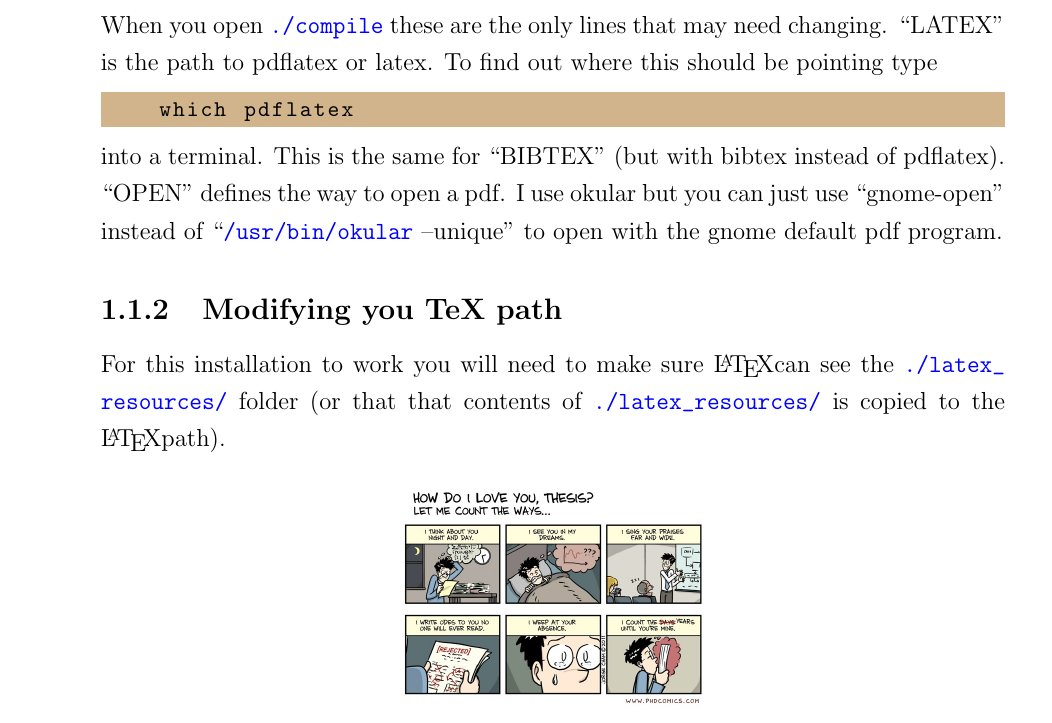
\includegraphics[width=\textwidth]{./figures/phd_comics_example.jpg}
    \\(a)
    \end{center}
    \end{minipage}
    \begin{minipage}{.49\textwidth}
    \begin{center}
    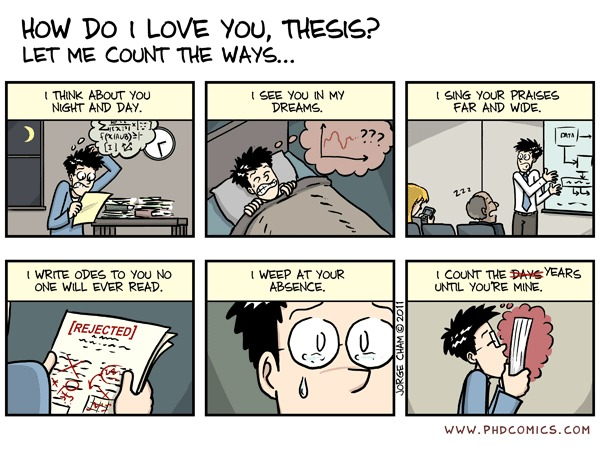
\includegraphics[width=\textwidth]{./footers/1.jpg}
    \\(b)
    \end{center}
    \end{minipage}
    \end{center}
    \caption[Short title for the list of figures]{Example side by side figure (a) The cartoon footer in the page (b) the jpg file in the \protect\url{./footers} folder. \label{ch1_figure_example_of_side_by_side}}
    \end{figure}

    \vspace{1cm}
    \noindent {\bf \textcolor{red}{NOTE: To turn off the cartoons (enabled by default) just comment out these lines in \url{./main.tex}.}}

    \begin{lstlisting}[style=base]

    @\fancyfoot@[C]{@\includegraphics@[@height@=4cm]
                   {./footers/\arabic{page}.jpg}}

    @\setlength@{@\textheight@}{22.5cm}

    \end{lstlisting}

%------------------------------------------------------------------------------------------------
\subsection{Indexing}
    \label{ch1_section_using_indexing}
%------------------------------------------------------------------------------------------------
    
    There are multiple ways to use the indexing. I use two commands to save on space.

    % This is just how I show code
    \begin{lstlisting}[style=base]
    @\define@{key}
    \end{lstlisting}

    displays the word in the text and adds it to the index. Note that keys are case sensitive and thus will appear multiple times in the index (define also auto capitalises index words so normally I just use the lowercase in the text)

    % This is just how I show code
    \begin{lstlisting}[style=base]
    @\defineas@{word}{key}
    \end{lstlisting}

    displays `word' in the text and adds a different word to the key. An example of when this may be useful is the case where you need a capital word in the text or a word such as `\defineas{photometric}{photometry}', where you only wish to have `\define{photometry}' in the index.

    \begin{lstlisting}[style=base]
    @\index@{key}
    \end{lstlisting}

    puts the key in the index. This requires you to put the word in the text separately.

    Examples of the use are below: 

    \begin{lstlisting}[style=base]
    The @\define@{star} was found by using the 
    @\defineas@{photometric}{photometry} bands, 
    this was useful to judge contamination 
    @\index@{contamination}.
    \end{lstlisting}

    This adds the words `\define{star}', `\define{photometry}' and `\define{contamination}' to the index (with a page reference to this page).

%------------------------------------------------------------------------------------------------
\subsection{Using the glossary}
    \label{ch1_section_using_glossary}
%------------------------------------------------------------------------------------------------

    I use a glossary to define terms such as \acro{2MASS}, \acro{WISE}, \acro{NIR} or \acro{SNR}.
    These words will only appear in the glossary when one of the following commands is used:

    % This is just how I show code
    \begin{lstlisting}[style=base]
    @\acro@{key}
    \end{lstlisting}

    displays the word in the text, and adds the key to the glossary and the index.

    \begin{lstlisting}[style=base]
    @\useglosentry@{key}
    \end{lstlisting} 

    adds the key only to the glossary only.


%------------------------------------------------------------------------------------------------
\subsection{Using acknowledgement citations}
    \label{ch1_section_using_acknowledgement_citations}
%------------------------------------------------------------------------------------------------

    This can be used in any \LaTeX \, document, basically reduces acknowledgements down in to citing the correct survey/telescope or word (acknowledgement terms are stored in \url{./preamble/acknowledgement_refs.tex})

    The can then be used anywhere (\ie at the end of a chapter) using the following command: 

    % This is just how I show code
    \begin{lstlisting}[style=base]
    @\acknowledge@{key}
    \end{lstlisting}

    an example of this is as follows:

    \begin{lstlisting}[style=base]
    @\acknowledge@{2MASS}
    @\acknowledge@{WISE}
    \end{lstlisting}

    And would produce the following text: \\

    \acknowledge{2MASS}

    \acknowledge{WISE}

    Note you can change the word `thesis' for all acknowledgements at the top of the \url{./preamble/acknowledgement_refs.tex} file.

    \subsubsection{Adding new acknowledgements}

    New acknowledgements are set up similar to bibtex files. In \url{./preamble/acknowledgement_refs.tex} keys are set up as follows:

    \begin{lstlisting}[style=base]
    @\pgfkeys@{/APLpy/.code = {This @\acknowledgetype@ made use of 
                               APLpy, an open-source plotting 
                               package for Python hosted at 
                               \url{http://aplpy.github.com}.}}
    \end{lstlisting}

    \noindent where
    \begin{lstlisting}[style=base]
    @\acknowledgetype@
    \end{lstlisting}

    \noindent is set near the start of \url{./preamble/acknowledgement_refs.tex}

    \begin{lstlisting}[style=base]
    \newcommand{\acknowledgetype}{@thesis@\,\,}
    \end{lstlisting}

    \noindent editing the text in red in the above will change all acknowledgements to use this instead of thesis (see above).



%------------------------------------------------------------------------------------------------
\subsection{Referencing Figures, Tables and Sections}
    \label{ch1_section_ref_fig_tab_sec}
%------------------------------------------------------------------------------------------------

    These are short cuts to writing ``Figure X'', ``Table Y'', ``Section Z'' and are edited in the \url{./preamble/newcommands.tex}.

    These are defined for a figure:

    % This is just how I show code
    \begin{lstlisting}[style=base]
    @\reffig@{reference}
    \end{lstlisting}

    \noindent the above is an alias of:

    \begin{lstlisting}[style=base]
    Figure @\ref@{reference}
    \end{lstlisting}

    A table:

    \begin{lstlisting}[style=base]
    @\reftab@{reference}
    \end{lstlisting}

    \noindent the above is an alias of:

    \begin{lstlisting}[style=base]
    Table @\ref@{reference}
    \end{lstlisting}

    And a section:

    \begin{lstlisting}[style=base]
    @\refsec@{reference}
    \end{lstlisting}

    \noindent the above is an alias of:

    \begin{lstlisting}[style=base]
    Section @\ref@{reference}
    \end{lstlisting}
    
    \noindent These aliases can be changed in \url{./preamble/newcommands.tex}:

    \begin{lstlisting}[style=base]
    %referencing sections, figures, tables, equations
    \newcommand{\reffig}[1]{@Figure@ \ref{#1}}
    \newcommand{\reftab}[1]{@Table@ \ref{#1}}
    \newcommand{\refequ}[1]{@Equation@ \ref{#1}}
    \newcommand{\refsec}[1]{@Section@ \ref{#1}}
    \end{lstlisting}

    \noindent \ie replacing Figure with Fig. will change every instance of reffig.

    An example of each is shown below:

    \begin{lstlisting}[style=base]
    \reffig{ch1_figure_1} shows x against y 
    (from \refsec{ch1_section_2}) and 
    is also shown in \reftab{ch1_table_3}.
    \end{lstlisting}

    This would give the following text:

    Figure 1 shows x against y (from Section 1.2) and is also shown in Table 3.
% Clear the page
\clearpage
% Chaper title
\chapter{The second chapter}
% Label for chapter
\label{ch2_second_chapter}
% Set the font size in this chapter
\normalsize
%===============================================================================
% Start of Chapter
%===============================================================================

%===============================================================================



\section{First section of Chapter 2}
    \label{ch2_section_first_section}


%===============================================================================


%===============================================================================



\section{First subsection of Chapter 2}
    \label{ch2_section_first_section_first_subsection}


%===============================================================================


%\include{./chapters/ch_3}
%\include{./chapters/ch_4}
%\include{./chapters/ch_5}
%\include{./chapters/ch_6}

%--------------------------------------------------------------------------%
%                                                                          %
%       The Bibliography, Glossary, Appendices and Index                   %
%                                                                          %
%--------------------------------------------------------------------------%

% Add references section
\newpage
\singlespacing
\phantomsection \label{references}
\addcontentsline{toc}{chapter}{References}
% set bib style
\bibliographystyle{./referencing/astroads}
% import bib file
\bibliography{./referencing/Bibliography.bib}

%--------------------------------------------------------------------------
% Add Glossary section
\newpage
\singlespacing
\phantomsection \label{listofglos}
\addcontentsline{toc}{chapter}{Glossary}
\printglossary

%--------------------------------------------------------------------------
% Add Appendix
\appendix
\chapter{Appendix A}
\label{ap:appA}

Test


%\chapter{Log of Observations}



%\appendixpage
%\addappheadtotoc

%--------------------------------------------------------------------------
% Add Index
\newpage
\singlespacing
\phantomsection \label{listofindex}
\addcontentsline{toc}{chapter}{Index}
\printindex

%--------------------------------------------------------------------------
% And we are done (now we just need to write the thesis)
\end{document}

%--------------------------------------------------------------------------%
%                                                                          %
%               END                                                        %
%                                                                          %
%--------------------------------------------------------------------------%
